\documentclass[12pt]{article}

%----------------------------------------------------------------------------------------
%   1. JASA & REQUIRED PACKAGES
%----------------------------------------------------------------------------------------
\usepackage{amsmath,amssymb,amsfonts} % Math packages
\usepackage{graphicx,psfrag,epsf}     % Graphics
\usepackage{enumerate}                % Lists
\usepackage{natbib}                   % Bibliography (JASA required)
\usepackage{url}                      % URLs

%----------------------------------------------------------------------------------------
%   2. YOUR PACKAGES (Retained from your file)
%----------------------------------------------------------------------------------------
\usepackage{amsthm}                   % Theorems
\usepackage{bbold}                    % Indicator functions etc
\usepackage{booktabs}                 % Professional tables
\usepackage{adjustbox}                % Box adjustments
\usepackage{subcaption}               % Subfigures
\usepackage{tikz}                     % Diagrams
\usetikzlibrary{arrows.meta}
\usepackage{algorithm}                % Algorithms
\usepackage{algorithmic}
\usepackage{listings}                 % Code listings
\usepackage{xcolor}                   % Colors

% SI Units setup
\usepackage{siunitx}
\sisetup{
  detect-mode,
  tight-spacing = true,
  table-number-alignment = center,
  group-digits = false
}

% Todo notes (Keep these for drafting, remove for final submission)
\usepackage{todonotes}
\usepackage{snaptodo}

% Hyperref (Loaded last to prevent conflicts)
\usepackage{hyperref}
\hypersetup{
  pdftitle={A General Marked Point Process Framework For Self-Exciting Network Evolution},
  pdfauthor={Clark; Kresin; Jones-Todd},
  colorlinks=true,
  linkcolor={blue},
  filecolor={Maroon},
  citecolor={Blue},
  urlcolor={Blue}
}

%----------------------------------------------------------------------------------------
%   3. JASA LAYOUT & MARGINS (DO NOT CHANGE)
%----------------------------------------------------------------------------------------
%\pdfminorversion=4
% NOTE: To produce blinded version, replace "0" with "1" below.
\newcommand{\blind}{1}

% JASA margins - 1 inch all around roughly
\addtolength{\oddsidemargin}{-.5in}%
\addtolength{\evensidemargin}{-.5in}%
\addtolength{\textwidth}{1in}%
\addtolength{\textheight}{-.3in}%
\addtolength{\topmargin}{-.8in}%

% JASA Spacing
\def\spacingset#1{\renewcommand{\baselinestretch}%
{#1}\small\normalsize} 

%----------------------------------------------------------------------------------------
%   4. YOUR MACROS & ENVIRONMENTS
%----------------------------------------------------------------------------------------
% Custom Macros
\def\AIC{\textsc{aic}}
\def\T{{ \mathrm{\scriptscriptstyle T} }}
\def\v{{\varepsilon}}
\DeclareMathOperator{\Thetabb}{\mathcal{C}}
\newcommand{\cmjt}[1]{{\color{blue}{#1}}}

% Theorem Environments
\newtheorem{example}{Example}
\newtheorem{theorem}{Theorem}[section]
\newtheorem{lemma}[theorem]{Lemma}
\newtheorem{proposition}[theorem]{Proposition}
\newtheorem{corollary}[theorem]{Corollary}
\newtheorem{assumption}[theorem]{Assumption}
\newtheorem{definition}[theorem]{Definition}
\newtheorem{remark}[theorem]{Remark}

% Listings setup
\lstset{
  basicstyle=\ttfamily\footnotesize,
  numbers=left,
  stepnumber=1,
  numbersep=5pt,
  frame=single,
  breaklines=true,
  language=Python
}

%----------------------------------------------------------------------------------------
%   DOCUMENT START
%----------------------------------------------------------------------------------------
\begin{document}

\bibliographystyle{agsm} % Using your requested style

% Initial spacing for title page
\spacingset{1}

%----------------------------------------------------------------------------------------
%   TITLE PAGE (JASA BLINDING LOGIC)
%----------------------------------------------------------------------------------------
\if1\blind
{
  \title{\bf A General Marked Point Process Framework For Self-Exciting Network Evolution}
  \author{Duncan A. Clark\thanks{
    The authors gratefully acknowledge \textit{funding sources here}.}\hspace{.2cm}\\
    Department of Statistics, Williams College\\
    and \\
    Conor J. Kresin \\
    Department of Mathematics and Statistics, University of Otago\\
    and \\
    Charlotte M. Jones-Todd\\
    Department of Statistics, University of Auckland}
  \maketitle
} \fi

\if0\blind
{
  \bigskip
  \bigskip
  \bigskip
  \begin{center}
    {\LARGE\bf A General Marked Point Process Framework For Self-Exciting Network Evolution}
\end{center}
  \medskip
} \fi

\bigskip

\begin{abstract}

We propose a novel modeling framework for time-evolving networks allowing for long-term dependence in network features that update in continuous time. Dynamic network growth is functionally parameterized via the conditional intensity of a marked point process. This characterization enables flexible, joint modeling of both update timing and the network updates themselves, dependent on the entire left-continuous sample path. We propose a path-dependent nonlinear marked Hawkes process as an expressive platform for modeling such data; its dynamic mark space embeds the time-evolving network. We establish stability conditions, demonstrate simulation and subsequent feasible likelihood-based inference through numerical study, and illustrate the methodology with an application to conference attendee social network data. The proposed formulation provides a flexible and principled foundation for statistical inference on complex network evolution in continuous time.
\end{abstract}

\section{Introduction}

Dynamic networks are well suited to modeling a variety of applications ranging from protein interaction \citep{jeong2001} to co-authorship \citep{newman2001}, economic behavior \citep{jackson2002evolution}, public health state laws \citep{clark2024}, and friendship networks \citep{lakon2014}. Such applications are characterized by a set of edges and nodes whose evolution exhibits complex temporal and network dependencies. There are many approaches to understanding the global properties of such networks, from early Erd\H{o}s--R\'enyi models \citep{erdos59}, to small-world models \citep{watts1998}, to scale-free approaches \citep{BA_model,BA_fitness_2001}, and densification over time \citep{Leskovec2005}. There are also approaches that seek to model bursty temporal networks; examples are found in \citet{sheng_bursty,holme_2012,holme_2015} and references therein. Such methods are useful for reproducing qualitative structure (centrality, path lengths, degree distributions, clustering), but they typically do not provide likelihood-based statistical inference for the mechanisms of network formation and growth.

Inference-focused dynamic network models often regard the node set as fixed and seek to understand the formation of edges over time. Examples include Stochastic Actor Oriented Models (SAOM) \citep{snijdersSAOM}, Temporal Exponential-family Random Graph models (TERGM) \citep{hanneke2010discrete}, Separable TERGM (STERGM) \citep{krivitsky_STERGM}, latent space Bayesian approaches \citep{Hoff2015}, and Latent Order Logistic models (LOLOG) \citep{Fellows2018}. These methods provide statistical inference on the edge formation process, but because the node set is typically treated as fixed, they do not facilitate inference on node arrivals in a growing network.

A central difficulty is that, in many settings, the times at which the network updates and the nature of those updates are not credibly independent \citep{snijders_2001}. Self-excitation in time is prevalent \cite{HuangLatentHawkes2022}: the arrival of a node or edge can increase the propensity for further updates in the near future. At the same time, network topology shapes which updates are plausible: preferential attachment, triadic closure, and other local mechanisms depend on the current network state. Capturing this joint dependence requires a continuous-time model in which update times and update content are jointly modelled.

Therefore, we propose a novel marked point process  \citep{daley2003introduction,kallenberg1976random} characterisation of time evolving networks: each network update corresponds to an event time, and the mark attached to that time is the update itself (the new nodes and edges added). This perspective allows a single conditional intensity characterisation for the coupled evolution of timing and topology. In this process, but because the node set is typically treated as fixed, they do not facilitate inference paper we focus on a Hawkesian ground specification \citep{Hawkes1971,hawkes1974cluster}, since self-excitation is a natural way to represent bursts of activity. However, the mark-space embedding that we propose is compatible with other point-process specifications. In particular, a marked point process viewpoint enables hitherto impossible statistical inference in this growing network setting, affording interpretability via complex parametric specifications.

Previous work connects point process and network modeling paradigms by treating node interaction data as realizations of continuous-time stochastic processes. For example, early relational event models \citep{Butts2008, VuHunterSmythAsuncion2011, HunterSmythVuAsuncion2011} and multivariate counting representations \citep{PerryWolfe2013} represent dynamic interactions  as collections of multivariate point processes indexed by dyads. However, these approaches do not explicitly model endogenous excitation through self-exciting intensity kernels as temporal dependence is primarily introduced via history statistics or time-varying covariates.


More recently, \citet{PassinoHeard2023} introduced mutually exciting point process graphs, where Hawkes-type intensities model the proposed self-exciting interaction dynamics on a fixed set of nodes, with intensities defined over dyads. Here, latent node parameters induce edge-specific baseline intensities and mutual excitation effects across dyads. Similarly \citep{HuangLatentHawkes2022} propose a latent space Hawkes formulation modeling how network structure and temporal excitation jointly influence node interactions through evolving latent positions, rather than through explicit stochastic network updates. The recent generative framework of \citep{Perez2025} attempts to characterize temporal networks, however they rely on a restrictive first-order Markovian assumption where the intensity is reduced to a function of the most recent event and a vector of hand-crafted features. In contrast, our framework avoids these simplifying losses of information, capturing the deep, long-term dependencies inherent in evolving network structures.

The closest precedent to our proposed framework is \citep{farajtabar2017coevolve}, where network updates are modeled via a joint conditional intensity and survival function in a multivariate Hawkes specification. While such work accommodates growth, inference on the network update mechanism is limited in that setting. The path-wise connection between univariate marked Hawkes processes and multivariate representations \citep{davis2024multivariate} provides a bridge to a large literature on multivariate Hawkes processes in network contexts, including mean-field limits \citep{delattre2016hawkes}, Hawkes graphs \citep{embrechts2018hawkes}, and latent group structure \citep{fang2024group}. We adopt a univariate marked formulation for parsimony: marks encode updates directly, avoiding the explosion of dimension that arises when treating each potential interaction type as a separate component.

The paper is structured as follows. Section~\ref{sec:prelim} introduces notation and the dynamic mark space encoding network updates. Section~\ref{sec:induced_models} presents our proposed "HawkesNet" models induced by network update PMFs and develops likelihood-based inference. Section~\ref{sec:path_dependent} introduces mark path dependent Hawkes processes and establishes stability results. Sections~\ref{sec:simulation_study} and \ref{sec:realdata} provide simulation studies and a real-data application. Section~\ref{sec:discuss} concludes, with proofs and additional examples in Appendix~\ref{sec:stability_theory}. All results in this paper were derived using the publicly available \texttt{hawkesNet} software package \cite{hawkesNest}.

% ======================================================================
\section{Dynamic Network Point Process Setup}\label{sec:prelim}
% ======================================================================


We consider a network at time $t$ to have  $N_t$ nodes, with edges represented by a binary matrix $A_t = \lbrace A_{i,j}^t \rbrace_{i=1,j=1}^{N_t}$ with $A^{t}_{i,j} \in \lbrace 0,1\rbrace$. The element $A_{i,j}^t$ is 0 if there is no edge between node $i$ and node $j$ and $1$ if the edge is present at time $t$. The network is defined as $\mathcal{G}_t = \lbrace N_t,A_{t} \rbrace $ at time $t$.


 Each edge and node in $\mathcal{G}_t$ has an associated "birth", defined as the earliest time it appears in the graph. $b_i = \inf(\lbrace t : i \leq N_t\rbrace)$ and $b_{i,j} = \inf(\lbrace t : A_{i,j}^{t} = 1\rbrace )$. At time $T$ we can therefore consider the node and edge arrival times $\mathcal{T}_{T} = \lbrace b_{j} : j\in {1\ldots N_T} \rbrace \cup \lbrace b_{j,k} : j,k \in {1\ldots N_T}  \rbrace$.

 We note that the $b_i$ and the $b_{i,j}$ edge arrivals may overlap, denoting an edge and a node being added to the network at the same time. Thus, we let $t_i \in \mathcal{T}_{T}$ the arrival time of the $i$th network update. This is now marked point process, see Section \ref{sec:mpp_notation} for precise specification. Each event is an update to the network, which allows both edges and nodes to be added at the same time, see Section \ref{sec:mpp_updates} for formal mark definitions.

\subsection{Marked point process notation}\label{sec:mpp_notation}

Following \citep{daley2007introduction}, a marked point process (MPP) is a $\mathbb{Z}^+$-valued random measure on a complete separable metric space (CSMS) $\mathcal X$. For the purposes of this paper, $\mathcal X=\mathbb{R}^+\times\mathcal{M}$, where $\mathcal{M}$ denotes the mark space. The MPP, $N$, has associated ground process $N_g(\cdot)$ which corresponds to temporal locations of points: $N_g(A)=N(A\times\mathcal M)$. We assume $N$ is locally finite and simple. On a bounded time window $[0,T)$ a realization consists of a finite set of tuples $\{(t_i,m_i)\}_{i=1}^{N([0,T)\times \mathcal M)}$. Let $\mathcal H_t$ be the natural history up to but not including time $t$, i.e.\ $\mathcal H_t=\sigma(N([0,t)\times B):B\subseteq \mathcal M)$.

The conditional intensity of $N$, denoted $\lambda$, is an integrable, nonnegative, $\mathcal{H}_t$-predictable process such that
\[
\mathbb{E}[N(dt,dm)\mid\mathcal H_t]=\lambda(t,m\mid\mathcal H_t)\,dt\,\nu(dm),
\]
where $\nu$ is a reference measure on $\mathcal M$. Since $\mathcal M$ will be discrete in our construction, the natural choice is counting measure.

 A point process is simple if, with probability one, all the points' spatiotemporal locations are distinct. We consider only simple point process estimation. Since the conditional intensity $\lambda$, uniquely determines the finite-dimensional distributions of any simple stationary point process (Proposition 7.2.IV of \cite{daley2003introduction}) we can model an MPP by specifying a model for $\lambda$. We note that growing networks themselves are often non-stationary; conveniently, the MPP characterisation itself is (see Section \ref{sec:path_dependent} for further discussion). 

Self-exciting point processes, where points in the past affect future intensity, can be modeled by Hawkes processes \citep{Hawkes1971}. A marked Hawkes process with background rate $\lambda_0(m)$ and triggering kernel $g$ is characterized in Definition \ref{def:mpp_hawkes}.

\begin{definition}[Marked Hawkes process]\label{def:mpp_hawkes}
Let $N$ be a simple marked point process on $\mathbb{R}_+ \times \mathcal{M}$ with
natural filtration $\{\mathcal{H}_t\}_{t \ge 0}$.  
We say that $N$ is a \emph{marked Hawkes process} if its
$\mathcal{H}_t$-conditional intensity admits the representation
\begin{equation}
\lambda(t,m \mid \mathcal{H}_t)
=
\lambda_{\emptyset}(t,m)
+
\int_{(0,t)\times\mathcal{M}}
g\!\left(t-u, m,m'\right)\,
N(du,dm'),
\label{eq:path_dependent_marked_hawkes}
\end{equation}
where $\lambda_{\emptyset}(t,m)$ is a predictable baseline intensity and
$g(t,m,m')$ is a predictable excitation kernel.
\end{definition}

Marked Hawkes processes are stationary when the offspring branching process is subcritical, i.e.\ the expected cluster size is finite (Lemma 6.3.II of \citealp{daley2007introduction}). Parameters of Hawkes intensities can be estimated consistently via maximum likelihood under standard conditions \citep{rathbun1996,schoenberg2016note,ogata1978estimators}.


For self-exciting network growth process, a network update at time $t$ depends on the current network as well as the timing and nature of previous updates. Such a process is termed non-separable. Often assumed for modelling simplicity, separability is imposed to facilitate likelihood computation \citep{davis2024multivariate,spassiani2024distribution}, and is not to be confused with the assumption of independent or unpredictable marks \citep{daley2007introduction}. Intuitively, a process is mark separable if the time process (corresponding to the ground process $N_g$, see \cite{daley2003introduction} for more details) and mark distribution can be decoupled after conditioning on history. This assumption restricts a rich class of models which require jointly considering how marks affect future event rates and vice-versa.

A non-separable specification is natural for the time-evolving random network growth process setting. For example, one may expect to wait a short time for an background singleton node to be added to the network but relatively long time for new highly connected node to arrive. For discussion and development of this idea see Section \ref{sec:path_dependent}.

\subsection{Network evolution as a marked point process}\label{sec:mpp_updates}

The network growth path $(\mathcal G_t)_{t\ge 0}$ is piecewise constant and changes only when new node(s) and/or edge(s) appear, we write $\mathcal G_{t-}$ for the left limit. At each $t_i$ we collect all new objects into a single mark $m_i$.

Let us consider a general space of possible updated to a network. Let $\mathcal V$ be a countably infinite set of possible node labels, and let $\mathcal E$ be the set of all potential edges on $\mathcal V$ (e.g.\ $\mathcal E=\{\{u,v\}:u,v\in\mathcal V,\ u\neq v\}$ for an undirected simple graph). Each event mark is a finite, nonempty subset
\[
m_i \subseteq \mathcal V \cup \mathcal E,
\qquad m_i\neq \emptyset,\quad |m_i|<\infty.
\]
Elements of $m_i\cap\mathcal V$ are the new nodes born at $t_i$, and elements of $m_i\cap\mathcal E$ are the new edges born at $t_i$. Edges in $m_i$ may connect pre-existing nodes and/or nodes introduced simultaneously in $m_i$.

The corresponding mark space is
\[
\mathcal M := \bigl\{m\subseteq \mathcal V\cup\mathcal E:\ m\text{ finite and nonempty}\bigr\}.
\]
Because $\mathcal V$ is countable, so is $\mathcal E$, and hence $\mathcal M$ is countable. Crucially, while $\mathcal M$ is fixed as a set, the admissible marks evolve with the current network state. Let $\mathcal M_t\subseteq\mathcal M$ denote the set of marks that correspond to valid additions given $\mathcal G_{t-}$ (e.g.\ no duplicate nodes/edges relative to $\mathcal G_{t-}$, and every edge endpoint is either already present at $t-$ or is introduced by the same mark). We enforce this dynamic admissibility through the conditional intensity by requiring
\[
\lambda(t,m\mid\mathcal H_t)=0 \qquad \text{for } m\notin \mathcal M_t.
\]
In practice one may further restrict $\mathcal M_t$ (e.g.\ by bounding how many nodes/edges may be added in a single update). Functionally we can understand this as a dynamic mark space, i.e. the space of possible updates to the network depends on the current network. This is a necessary contrast to typical marked point processes. For example the typical spatiotemporal point process has a fixed $\mathbb{R}^{2}$ mark space.

We can naturally define admissible node and edge sets sets just before time $t$, $\mathcal V_{G_{t-}}$ and $\mathcal E_{G_{t-}}$ via $\mathcal M_t := \bigl\{m\subseteq \mathcal V_t\cup\mathcal E_t \bigr\}$.

This construction makes the key identification used throughout the paper: the evolving network and the marked update sequence are two views of the same object. Given an initial graph $(V_0,E_0)$, the node and edge sets at time $t$ are obtained by accumulating marks,
\[
V_t = V_0 \,\cup\, \bigcup_{i:\,t_i\le t}\bigl(m_i\cap\mathcal V_{G_{t-}}\bigr),
\qquad
E_t = E_0 \,\cup\, \bigcup_{i:\,t_i\le t}\bigl(m_i\cap\mathcal E_{G_{t-}}\bigr),
\]

Thus $\mathcal G_t$ is determined by $\{(t_i,m_i):t_i\le t\}$. Conversely, the jump times and jump sizes of $(\mathcal G_t)$ define the marked update sequence.

We observe updates $\{(t_i,m_i)\}_{i=1}^n$ on $[0,T)$. We represent them as a simple marked point process
$N=\sum_{i=1}^n \delta_{(t_i,m_i)}$ on $\mathbb R^+\times\mathcal M$, with history $\mathcal H_t$ and (predictable) conditional intensity
$\lambda(t,m\mid\mathcal H_t)$ w.r.t.\ $dt\,\nu(dm)$ (here $\nu$ is counting measure on the countable $\mathcal M$).
Admissibility is enforced by $\lambda(t,m\mid\mathcal H_t)=0$ for $m\notin\mathcal M_t$. Note that the simplicity of the process is ensured by regarded network updates as marks, not simply restricting to adding single edges or nodes as events.

\section{Network probability mass function induced models}\label{sec:induced_models}

Specifying the types of network updates that are likely is crucial to appropriately modeling network evolution. Within our framework, a convenient way to specify a (possibly non-separable) marked intensity on the countable mark space $\mathcal M$ is via the factorization
\begin{equation}\label{eq:lambda_factor_induced}
\lambda(t,m\mid\mathcal H_t)=\lambda_g(t\mid\mathcal H_t)\,q(m\mid t,\mathcal H_t),
\end{equation}
where $\lambda_g(t\mid\mathcal H_t)=\sum_{m\in\mathcal M}\lambda(t,m\mid\mathcal H_t)$ is the ground rate and $q(\cdot\mid t,\mathcal H_t)$ is a PMF supported on the admissible set $\mathcal M_t$.
We call any model built by combining a ground-rate specification for $\lambda_g$ with a network-growth PMF $q$ a HawkesNet model. Even if $q$ does not depend explicitly on $t$, the resulting model need not be separable because the support $\mathcal M_t$ and the features entering $q$ evolve with the graph.

We consider two examples of induced models. The Barabasi Albert (BA) preferential attachment model \citep{BA_model}, is widely used to account for power law behaviour observed in many networks' degree distributions.

\begin{example}[Preferential Attachment HawkesNet]\label{ex:BA}

We can formulate a two-parameter $(\tau, m)$ BA-style induced kernel with time decay. The parameter $\tau > 0$ controls the rate of decay of past degrees; $m > 0$ is the expected number of edges added at each event. At event time $t$, the mark $m_t$ is drawn as follows: (i) add one new node at time $t$; (ii) draw the number of edges to add, $K_t$, from a distribution with mean $m$ (e.g., $K_t \sim \text{Poisson}(m)$), and set $K_t \leftarrow \min(K_t, N_{t-})$ so that at most $N_{t-}$ edges are added; (iii) connect the new node to $K_t$ distinct existing nodes by sampling without replacement according to the BA attachment probabilities below. Thus $m$ governs the growth in degree per event, while $\tau$ governs how much older nodes are down-weighted relative to degree.

The probability that an existing node $i$ is chosen as an attachment target (given the history $\mathcal{H}_t$) is
\begin{align*}
p_i^{\text{BA}} = \frac{\delta_i}{\sum_{k=1}^{N_{t-}} \delta_k},
\end{align*}
where $\delta_i^t = \exp(-\tau (t - t_i)) \cdot d_i^t$, and $d_i^t$ is the degree of node $i$ immediately before time $t$. This yields preferential-attachment behavior with time decay, and $\delta_i^t$ plays the role of a time-decayed ``fitness'' in the extended BA framework \citep{BA_fitness_2001}. Let $\mathcal{E}(m_t)$ denote the edge set of the mark $m_t$, and define $e_i = \mathbb{I}\bigl((N_{t-}+1, i) \in \mathcal{E}(m_t)\bigr)$. Proceeding edgewise and assuming independence between edges of the update, the mark density can be written as the product of the marginal distribution for $K_t$ (e.g., $\text{Poisson}(K_t; m)$) and a product of Bernoulli terms over the $N_{t-}$ possible targets:
\begin{align}\label{eq:bernoulli}
q(m_t \mid t, \mathcal{H}_t) = \mathbb{P}(K_t \mid m) \times \prod_{i=1}^{N_{t-}} \bigl(p_i^{\text{BA}}\bigr)^{e_i} \bigl(1 - p_i^{\text{BA}}\bigr)^{1-e_i}.
\end{align}
Here $\sum_{i=1}^{N_{t-}} e_i = K_t$, and the product encodes the probability of the observed edge set under the BA rule; the Poisson factor explicitly ties the number of edges per event to the parameter $m$.
\end{example}

The BA model simply adds nodes to well-connected nodes, independently of other structure in the network. For social networks, where existing, complex network structure may be considered to impact the probability of an edge being added, this is insufficient. We also consider the change statistic model as an alternative model that can consider complex network structure.

\begin{example}[Change Statistic HawkesNet]\label{ex:cs}

For a network $y$ and a vector of network statistics $g(y) \in \mathbb{R}^{p}$, the change statistic for an update $m$ is $C(m) = g(y^{m+}) - g(y^{m-})$, where $y^{m+}$ is the network $y$ with the update $m$ applied and $y^{m-}$ is the network without that update. Change statistics thus measure the effect of an update on arbitrary network statistics. A mark PMF can be induced by adding edges according to a logistic model on these change statistics, following the Exponential-family Random Graph Model (ERGM) literature \citep{FrankStrauss1986,snijders2006,Robins2007} and related network growth models \citep{Fellows2018}.

For a single candidate edge $(i,j)$, write $C_{i,j} = g(y_{i,j}^{+}) - g(y_{i,j}^{-})$, where $y_{i,j}^{+}$ is $y$ with edge $(i,j)$ and $y_{i,j}^{-}$ is $y$ without it. For example, if $g(y) = (\text{edge count}(y), \text{triangle count}(y))^{\top}$, then $C_{i,j}$ has first component $1$ and second component equal to the number of triangles that edge $(i,j)$ would complete.

We define a two-step procedure for drawing the mark $m_t$ at event time $t$. Let $\theta \in \mathbb{R}^{p}$ be the parameter vector for the change statistics, $\tau > 0$ the time-decay rate, and $\lambda > 0$ the expected number of new nodes per event. (1) Draw the number of new nodes, $N_t^{\text{new}}$, from $\text{Poisson}(\lambda)$ and add these nodes at time $t$. (2) Restrict to candidate edges between the new nodes and existing nodes (or a time-truncated subset of existing nodes), so that the number of candidate edges is $\mathcal{O}(n)$ rather than $\mathcal{O}(n^2)$. For each candidate edge $(i,j)$, the probability of adding the edge is
\begin{equation}\label{eqn:csdraw}
p_{i,j}^{\text{CS}} = \exp\bigl(-\tau \cdot (t - t_i)\bigr) \cdot \frac{1}{1 + \exp(-\theta^{\top} C_{i,j})},
\end{equation}
where $t_i$ is the time of the most recent activity of node $i$ (e.g., its arrival time). Thus $\tau$ down-weights older nodes relative to the logistic term. Under the approximation that edge indicators are conditionally independent given the network history, the mark density factors as the Poisson mass for $N_t^{\text{new}}$ times a product of Bernoulli terms over the candidate edges, as in the BA case (\ref{eq:bernoulli}):
\begin{equation}\label{eq:csdensity}
q(m_t \mid t, \mathcal{H}_t) = \text{Poisson}(N_t^{\text{new}}; \lambda) \times \prod_{(i,j) \in \mathcal{C}_t} \bigl(p_{i,j}^{\text{CS}}\bigr)^{e_{i,j}} \bigl(1 - p_{i,j}^{\text{CS}}\bigr)^{1 - e_{i,j}},
\end{equation}
where $\mathcal{C}_t$ is the set of candidate edges at time $t$ and $e_{i,j} = \mathbb{I}\bigl((i,j) \in \mathcal{E}(m_t)\bigr)$. Optionally, discrete vertex attributes on new nodes can be modeled with an accompanying model (see Appedix \ref{app:gender}). Restricting candidates to new-to-old edges (and optionally to the most recent nodes under truncation) keeps the number of terms in the product $\mathcal{O}(n)$ and makes the procedure feasible as $n$ grows.
\end{example}

There is significant work on similar models \cite{Fellows2018,lusher2012} with social theory driving the selection of suitable statistics \cite{snijders2006}. The model is specified by the choice of network statistics, common choices include triangles for modeling transitive closure, as well as k-stars, (a single node connected to $k$ others) to model node popularity. One can also consider nodal covariate  based statistics, for example gender, one could then consider the count of matched gender edges, or other related statistics. The inclusion of structural and nodal covariate statistics allows for inference on the nodal covariate, while also accounting for the tendency towards transitive closure.

\begin{remark}
    Including the triangle term induces global dependence among all edges. This leads to related issues of near degeneracy \citep{handcock2003} where significant probability mass is places on empty and complete networks. However, our inclusion of the time decay term mitigates this as the global dependence diminishes over time, a full investigation of degeneracy is beyond the scope of this work.
\end{remark}

\section{Mark path dependent Hawkes processes}\label{sec:path_dependent}
% ======================================================================

We focus on modeling the ground process as a marked Hawkes process, with our novel dynamic mark space. We next explore the consequences with regard to the cluster representation of the proposed MPP and develop theory for existence, uniqueness and non-explosion of the MPP. 

Linear Hawkes processes admit a Poisson cluster representation \citep{hawkes1974cluster} in which immigrant points generate independent offspring according to the triggering kernel. This additivity implies that the contribution of any single point to the future intensity is fixed at its birth and does not change later. That picture is often ill-suited for network growth when excitation depends on evolving topology. For instance, an edge created early may later become part of many triangles; if excitation depends on such motifs, then the impact of that old edge on the current intensity depends on the \emph{current} network, not only on the mark at its creation.

\begin{figure}[!htb]
    \centering
    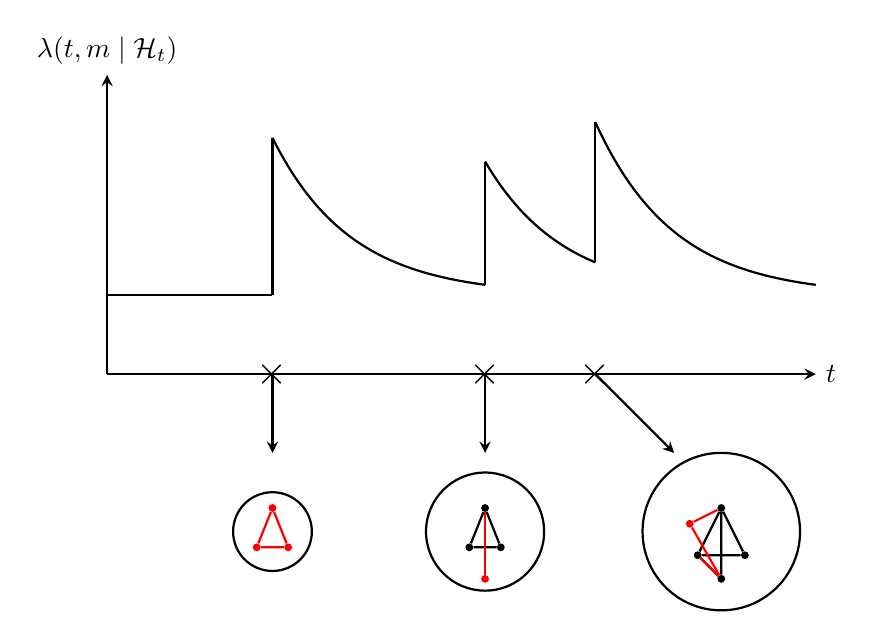
\begin{tikzpicture}[>=stealth,thick,scale=1.0]

\draw[->] (0,0) -- (0,3.8) node[above] {\(\lambda(t,m\mid\mathcal{H}_t)\)};
\draw[->] (0,0) -- (9,0)   node[right] {\(t\)};

\def\tOne{2.1}
\def\tTwo{4.8}
\def\tThree{6.2}
\def\baseline{1}

\draw[thick] (0,\baseline) -- (\tOne,\baseline);
\draw[thick] (\tOne,\baseline) -- (\tOne,3);
\draw[thick,domain=\tOne:\tTwo,samples=60,smooth]
  plot(\x,{ (3 - \baseline)*exp(-( \x - \tOne)) + \baseline });
\pgfmathsetmacro{\valAtTTwo}{
  (3 - \baseline)*exp(-( \tTwo - \tOne)) + \baseline
}
\draw[thick] (\tTwo,\valAtTTwo) -- (\tTwo,2.7);
\draw[thick,domain=\tTwo:\tThree,samples=60,smooth]
  plot(\x,{ (2.7 - \baseline)*exp(-( \x - \tTwo)) + \baseline });
\pgfmathsetmacro{\valAtTThree}{
  (2.7 - \baseline)*exp(-( \tThree - \tTwo)) + \baseline
}
\draw[thick] (\tThree,\valAtTThree) -- (\tThree,3.2);
\draw[thick,domain=\tThree:9,samples=60,smooth]
  plot(\x,{ (3.2 - \baseline)*exp(-( \x - \tThree)) + \baseline });

\node at (\tOne,0) {\Large $\times$};
\node at (\tTwo,0) {\Large $\times$};
\node at (\tThree,0) {\Large $\times$};

\draw[->] (\tOne,0)   -- (\tOne,-1);
\draw[->] (\tTwo,0)   -- (\tTwo,-1);
\draw[->] (\tThree,0) -- (\tThree+1,-1);

\draw (\tOne,-2) circle (.5);
\node[circle,fill=red,scale=0.3] (a1) at (\tOne-0.2,-2.2) {};
\node[circle,fill=red,scale=0.3] (a2) at (\tOne+0.0,-1.7) {};
\node[circle,fill=red,scale=0.3] (a3) at (\tOne+0.2,-2.2) {};
\draw[red] (a1) -- (a2) -- (a3) -- (a1);

\draw (\tTwo,-2) circle (.75);
\node[circle,fill=black,scale=0.3] (b1) at (\tTwo-0.2,-2.2) {};
\node[circle,fill=black,scale=0.3] (b2) at (\tTwo+0.0,-1.7) {};
\node[circle,fill=black,scale=0.3] (b3) at (\tTwo+0.2,-2.2) {};
\draw (b1) -- (b2) -- (b3) -- (b1);
\node[circle,fill=red,scale=0.3] (b4) at (\tTwo,-2.6) {};
\draw[red] (b2) -- (b4);

\draw (\tThree+1.6,-2) circle (1);
\node[circle,fill=black,scale=0.3] (c1) at (\tThree+1.3,-2.3) {};
\node[circle,fill=black,scale=0.3] (c2) at (\tThree+1.6,-1.7) {};
\node[circle,fill=black,scale=0.3] (c3) at (\tThree+1.9,-2.3) {};
\node[circle,fill=black,scale=0.3] (c4) at (\tThree+1.6,-2.6) {};
\draw (c1) -- (c2) -- (c3) -- (c1) -- (c4) -- (c2);
\node[circle,fill=red,scale=0.3] (c5) at (\tThree+1.2,-1.9) {};
\draw[red] (c4) -- (c5);
\draw[red] (c2) -- (c5);
\draw[red] (c4) -- (c1);

\end{tikzpicture}
    \caption{A nonlinear Hawkes representation of network-update data. Red edges and nodes represent the mark at each event. The black bubbles represent the accumulated network state. As the network evolves, the effect of old edges on triggering can change as their embedding (e.g.\ triangle participation) changes over time.}
    \label{fig:networkHawkes}
\end{figure}

\begin{figure}[!htb]
\centering

% --- local colors/styles for this figure ---
\colorlet{mpdcol}{red!55!blue} % "purple" mix
\tikzset{
  highlight/.style={draw=black, line width=0.6pt, minimum width=18pt, minimum height=18pt, inner sep=1pt},
  branch/.style={->, line width=0.9pt},
  histdep/.style={->, mpdcol, line width=0.9pt}
}

\begin{subfigure}[b]{0.47\textwidth}
\centering
\begin{tikzpicture}[>=stealth,scale=0.72,transform shape]
\draw (0,0) -- (10,0);

% events on the time line (cluster schematic)
\node[blue] (leftO) at (0,0) {\Large O};
\node[blue] (x1)    at (2,0) {\Large X};
\node[blue] (x2)    at (3,0) {\Large X};

\node[red]  (midO)  at (5,0) {\Large O};
\node[red]  (rx1)   at (6,0) {\Large X};
\node[red]  (rx2)   at (7,0) {\Large X};

\node[blue,highlight] (boxX) at (9,0) {\Large X};

% one possible branching/parent assignment (Poisson cluster representation)
\draw[branch,blue] (leftO.north) .. controls (1,1.2) .. (x1.north);
\draw[branch,blue] (leftO.north) .. controls (2,1.6) .. (x2.north);
\draw[branch,blue] (leftO.north) .. controls (6,2.2) .. (boxX.north);

\draw[branch,red]  (midO.north)  .. controls (5.5,1.1) .. (rx1.north);
\draw[branch,red]  (midO.north)  .. controls (6.2,1.4) .. (rx2.north);
\end{tikzpicture}
\caption{Linear Hawkes (Poisson cluster view).}
\label{fig:linearHawkes}
\end{subfigure}
\hfill
\begin{subfigure}[b]{0.47\textwidth}
\centering
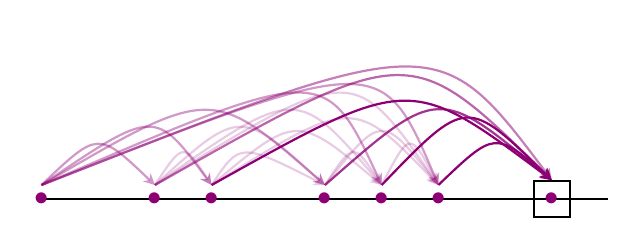
\begin{tikzpicture}[>=stealth,thick,scale=0.72,transform shape]
\colorlet{purple}{red!55!blue} % "purple" mix
\draw (0,0) -- (10,0);
\node[purple] (leftO) at (0,0) {\Large $\bullet$};
\node[purple] (x1) at (2,0) {\Large $\bullet$};
\node[purple] (x2) at (3,0) {\Large $\bullet$};
\node[purple] (midO) at (5,0) {\Large $\bullet$};
\node[purple] (rx1) at (6,0) {\Large $\bullet$};
\node[purple] (rx2) at (7,0) {\Large $\bullet$};
\node[purple, draw=black, thick, minimum width=18pt, minimum height=18pt] (boxX) at (9,0) {\Large $\bullet$};

% blue arrows from leftO
\draw[->,purple, opacity=0.4] (leftO.north) .. controls (1,1.2) .. (x1.north);
\draw[->,purple, opacity=0.4] (leftO.north) .. controls (2,1.6) .. (x2.north);
\draw[->,purple, opacity=0.4] (leftO.north) .. controls (3,2.0) .. (midO.north);
\draw[->,purple, opacity=0.4] (leftO.north) .. controls (5,2.4) .. (rx1.north);
\draw[->,purple, opacity=0.4] (leftO.north) .. controls (6,2.6) .. (rx2.north);
\draw[->,purple, opacity=0.5] (leftO.north) .. controls (7,3.0) .. (boxX.north);

% purple arrows from x1
\draw[->,purple, opacity=0.2] (x1.north) .. controls (2.5,1.0) .. (x2.north);
\draw[->,purple, opacity=0.2] (x1.north) .. controls (3.5,1.6) .. (midO.north);
\draw[->,purple, opacity=0.2] (x1.north) .. controls (4.5,2.0) .. (rx1.north);
\draw[->,purple, opacity=0.2] (x1.north) .. controls (5.5,2.4) .. (rx2.north);
\draw[->,purple, opacity=0.6] (x1.north) .. controls (6.5,2.8) .. (boxX.north);

% purple arrows from x2
\draw[->,purple, opacity=0.2] (x2.north) .. controls (3.5,1.0) .. (midO.north);
\draw[->,purple, opacity=0.2] (x2.north) .. controls (4.5,1.5) .. (rx1.north);
\draw[->,purple, opacity=0.2] (x2.north) .. controls (5.5,1.8) .. (rx2.north);
\draw[->,purple, opacity=1] (x2.north) .. controls (6.5,2.2) .. (boxX.north);

% red arrows from midO
\draw[->,purple, opacity=0.2] (midO.north) .. controls (5.5,1.0) .. (rx1.north);
\draw[->,purple, opacity=0.2] (midO.north) .. controls (6.0,1.5) .. (rx2.north);
\draw[->,purple, opacity=0.8] (midO.north) .. controls (7.0,2.0) .. (boxX.north);

% red arrows from rx1
\draw[->,purple, opacity=0.2] (rx1.north) .. controls (6.5,1.2) .. (rx2.north);
\draw[->,purple, opacity=1] (rx1.north) .. controls (7.5,1.8) .. (boxX.north);

% red arrows from rx2
\draw[->,purple, opacity=1] (rx2.north) .. controls (8.0,1.2) .. (boxX.north);
\end{tikzpicture}
\caption{Mark path-dependent (nonlinear).}
\label{fig:nonlinearHawkes}
\end{subfigure}

\caption{Contrasting dependence structures in Hawkes models.
\textbf{(a)} In a linear marked Hawkes process, the Poisson cluster representation implies that, conditional on a latent parent/branching assignment (arrows), clusters (colors) can be generated independently; $O$ denotes an immigrant and $X$ denotes an offspring.
\textbf{(b)} In a mark path-dependent Hawkes process, the mark at time $t$ may depend on the entire marked history (e.g., through the current network state and the time-varying admissible mark set $\mathcal M_t$). We therefore depict history dependence of the boxed event via fan-in arrows from all past events; these arrows are \emph{not} a branching genealogy. Using a single (mixed) color emphasizes the lack of a cluster decomposition, and arrow opacity schematically represents relative influence (e.g., stronger for more recent events under temporal decay).}
\label{fig:hawkes_linear_vs_nonlinear}
\end{figure}




As discussed in Section~\ref{sec:mpp_notation}, a common simplification for marked point processes is mark separability, which informally asks that (conditional on history) the mechanism governing when events occur can be decoupled from the mechanism governing what update occurs. For dynamic networks, mark separability is often too restrictive. The reason is that the current topology simultaneously affects (i) the short-term propensity for any update to occur and (ii) which specific updates are plausible. For example, if excitation depends on motifs (triangles, $k$-stars, shared partners), then the same past edge can become more (or less) excitable as the surrounding network evolves. In that case, the timing mechanism and the mark mechanism are inherently entangled: a topology-altering update can change the short-term event rate, while the burst regime (high $\lambda_g$) can change which marks are likely.

This motivates working with a genuinely non-separable marked intensity,
\begin{equation}
\label{eq:non_sep_mpd}
\lambda(t,m\mid\mathcal H_t)=f(t,m,\mathcal H_t),
\end{equation}
that cannot be reduced to a decoupled form without losing the topology--timing feedback that is central in growth settings.

For later likelihood and thinning calculations it is convenient to define the ground rate and conditional mark PMF
\[
\lambda_g(t\mid\mathcal H_t):=\sum_{m\in\mathcal M}\lambda(t,m\mid\mathcal H_t),
\qquad
q(m\mid t,\mathcal H_t):=\frac{\lambda(t,m\mid\mathcal H_t)}{\lambda_g(t\mid\mathcal H_t)}\ \ (\lambda_g>0).
\]
This identity is purely algebraic, in our setting both $\lambda_g$ and $q$ may depend on the full marked history (through the evolving graph), so it does not impose mark separability.

We will proceed using Hawkes processes, concretely we define the mark path dependent Hawkes process as follows:

\begin{definition}[Mark path-dependent Hawkes process]\label{def:mpd}
Let $N$ be a simple marked point process on $\mathbb{R}_+ \times \mathcal{M}$ with
natural filtration $\{\mathcal{H}_t\}_{t \ge 0}$.  
We say that $N$ is a \emph{mark path-dependent Hawkes process} if its
$\mathcal{H}_t$-conditional intensity admits the representation
\begin{equation}
\lambda(t,m \mid \mathcal{H}_t)
=
\lambda_{\emptyset}(t,m)
+
\int_{(0,t)\times\mathcal{M}}
g\!\left(t-u, m, m' \mid \mathcal{H}_t\right)\,
N(du,dm'),
\label{eq:path_dependent_marked_hawkes}
\end{equation}
where $\lambda_{\emptyset}(t,m)$ is a predictable baseline intensity and
$g(t,m, m' \mid \mathcal{H}_t)$ is a predictable excitation kernel.
\end{definition}

This yields the more intuitive, yet equivalent sum representation in which past contributions to the intensity may depend on the current mark as well as the current history:
\begin{equation}\label{eq:condintenHN}
    \lambda(t,m\mid\mathcal H_t)=\lambda_{\emptyset}(t,m)+\sum_{i:t_i<t}g(t-t_i,m,m_i\mid\mathcal H_t).
\end{equation}

Definition \ref{def:mpd} differs from Definition \ref{def:mpp_hawkes}, in that the excitation kernel depends on the full history, inducing the non linearity as discussed above. The nonlinearity here is not an external ``activation function'' applied uniformly to the integrated past; rather it is embedded inside each kernel term through path dependence on the current network state. This is exactly what occurs when the effect of an old edge depends on network statistics (triangles, stars, centrality, etc.) that can change after the edge is born.

At first glance, conditioning $g(\cdot\mid\mathcal H_t)$ on $\mathcal H_t$ (rather than on $\mathcal H_{t_i}$) can look like it violates causality, since the contribution of an event at time $t_i$ is evaluated using information after $t_i$. In the network setting this is the natural interpretation: as the network evolves, the ``excitement potential'' of past edges and nodes can change as they become embedded in a denser or more clustered topology. Figure~\ref{fig:networkHawkes} visualizes this interpretation directly: red elements denote the \emph{current update mark}, while the black ``bubble'' is the cumulative network state on which the next intensity evaluation is based. In contrast to the fixed offspring structure in Figure~\ref{fig:linearHawkes}, the contribution of older updates can change as the black state evolves, matching the intuition behind Figure~\ref{fig:nonlinearHawkes}.

For likelihood-based inference, the model must define a well-posed stochastic process. Existence ensures that the intensity specification corresponds to at least one marked point process; uniqueness ensures that the specification does not admit multiple incompatible laws; and non-explosion ensures that on any finite time window there are almost surely only finitely many updates. These properties are not merely mathematical housekeeping. In practice, explosion would make simulation unstable, likelihood integrals ill-defined, and parameter estimates uninterpretable. Uniqueness is what allows us to interpret fitted parameters as identifying a single data-generating mechanism rather than a family of possibilities with the same formal intensity expression.

For mark path dependent Hawkes processes, cluster-based arguments are not available in general, so the usual linear-Hawkes branching construction is not the right tool. Instead we work with the Poisson-embedding (thinning) representation and a contraction argument in a natural metric on marked histories. Intuitively, the key requirement is that changing the past by adding or removing a single event can only affect the current intensity by an amount that decays with that event’s age, and that these effects are sufficiently summable over time. This is precisely what explicit time decay (aging) and bounded local update mechanisms enforce in the induced network models in Section~\ref{sec:induced_models}.

\subsection{Poisson embedding and simulation via thinning}\label{sec:poisson_embedding}

The Poisson embedding is the common engine behind (i) the fixed-point definition of the model, (ii) existence/uniqueness and non-explosion proofs via contraction, and (iii) exact simulation by thinning. The logic is as follows, specify an intensity functional $\eta\mapsto \lambda(\cdot,\cdot\mid\eta)$ on marked histories, embed it into a single Poisson random measure, and then construct the process as a self-consistent thinning of that Poisson measure \citep{bremaud1996stability}.

Let $\Pi$ be a Poisson random measure on $E=\mathbb R\times\mathbb R_+\times\mathcal M$ with intensity $dt\,dz\,\nu(dm)$, where $\nu$ is counting measure on $\mathcal M$. Given a predictable marked intensity $\lambda(t,m\mid\mathcal H_t)$, define a marked point process by thinning:
\begin{equation}\label{eq:thinning}
N(dt,dm)=\int_{\mathbb R_+}\mathbf 1\{z\le \lambda(t,m\mid\mathcal H_t)\}\,\Pi(dt,dz,dm).
\end{equation}
Equation \eqref{eq:thinning} is both the stochastic fixed-point equation defining the process and (after choosing a dominating proposal rate) the basis for simulation by thinning.

We state assumptions directly on the full marked intensity functional $\eta\mapsto \lambda(\cdot,\cdot\mid\eta)$, where $\eta$ is a generic marked history (an integer-valued measure on $\mathbb R\times\mathcal M$). 

\begin{assumption}[Bounded baseline]\label{ass:H0}
Let $\mathbf 0$ denote the empty history. Define $\lambda_{\emptyset}(t,m):=\lambda(t,m\mid\mathbf 0)$ and $\lambda_{g,\emptyset}(t):=\sum_m \lambda_{\emptyset}(t,m)$. Assume $\sup_{t\in\mathbb R}\lambda_{g,\emptyset}(t)<\infty$.
\end{assumption}

\begin{assumption}[Marked Lipschitz contraction]\label{ass:HL}
There exists measurable $h:\mathbb R_+\to\mathbb R_+$ with $\int_0^\infty h(u)\,du<1$ such that for all $t\in\mathbb R$ and histories $\eta,\eta'$,
\[
\sum_{m\in\mathcal M}\bigl|\lambda(t,m\mid\eta_t)-\lambda(t,m\mid\eta'_t)\bigr|
\le
\int_{(-\infty,t)\times\mathcal M} h(t-s)\,|\eta-\eta'|(ds,dm),
\]
where $|\eta-\eta'|$ is total variation (symmetric-difference count for integer-valued measures), and $\eta_t$ is the restriction of $\eta$ to $(-\infty,t)\times\mathcal M$.
\end{assumption}

\begin{assumption}[Time-shift covariance]\label{ass:shift}
Let $\theta_u$ denote time-shift on histories: $(\theta_u\eta)(A\times B)=\eta((A+u)\times B)$. Assume there exists a measurable functional $\Lambda$ such that $\lambda(t,m\mid\eta_t)=\Lambda_m(\theta_t\eta)$ for all $t$ and $m$.
\end{assumption}

\begin{theorem}[Existence, pathwise uniqueness, non-explosion]\label{thm:existence}
Assume \ref{ass:H0}--\ref{ass:HL}. Then there exists a pathwise unique simple marked point process $N$ on $[0,\infty)\times\mathcal M$ satisfying the fixed-point thinning equation \eqref{eq:thinning}. Moreover, for every $T>0$, $\mathbb E[N([0,T]\times\mathcal M)]<\infty$, hence $N([0,T]\times\mathcal M)<\infty$ almost surely.
\end{theorem}

\begin{proof}[(Proof sketch):] The fixed-point map in \eqref{eq:thinning} is a \emph{thinning map}: given a candidate history $\eta$, one can thin $\Pi$ using $\lambda(\cdot,\cdot\mid \eta)$ to produce a new history. The proof iterates this map (Picard iteration), coupling all iterates using the \emph{same} Poisson random measure $\Pi$. A basic thinning-coupling inequality shows that the expected symmetric-difference count of two coupled thinnings on $[0,T]$ is bounded by the time integral of the $\ell^1(\mathcal M)$ distance between their intensities. Assumption~\ref{ass:HL} then converts intensity discrepancy into a weighted count of past mismatched events. The condition $\int_0^\infty h(u)\,du<1$ makes this a contraction on each finite horizon, yielding a Cauchy sequence of iterates and therefore existence of a limit process. Pathwise uniqueness follows by applying the same contraction argument to any two putative solutions driven by the same $\Pi$. 

Once a solution exists, Assumption~\ref{ass:HL} bounds the ground intensity $\lambda_g(t)=\sum_m \lambda(t,m\mid\mathcal H_t)$ by the baseline rate plus a convolution of $h$ with the counting process itself. Taking expectations yields an integral inequality for $\mathbb E[\lambda_g(t)]$ whose supremum is bounded by $(1-\|h\|_1)^{-1}\sup_t \lambda_{g,\emptyset}(t)$. Integrating over $[0,T]$ implies $\mathbb E[N([0,T]\times\mathcal M)]<\infty$, which rules out explosion (if $N([0,T]\times\mathcal M)=\infty$ with positive probability, the expectation would be infinite).\end{proof}

\begin{theorem}[Stationary ergodic marked solution]\label{thm:stationary}
Assume \ref{ass:H0}--\ref{ass:HL}--\ref{ass:shift}. Then there exists a stationary marked point process $N^{\mathrm{stat}}$ on $\mathbb R\times\mathcal M$ satisfying \eqref{eq:thinning} for all $t\in\mathbb R$, and its law is unique among stationary solutions. Moreover, $N^{\mathrm{stat}}$ is ergodic under time shifts.
\end{theorem}

\begin{proof}[(Proof sketch):] Time-shift covariance (Assumption~\ref{ass:shift}) makes the fixed-point thinning map time-homogeneous on $\mathbb R$. One then couples (i) the stationary candidate constructed from an infinite past and (ii) the process started from empty history at time $0$, again using the same $\Pi$, and shows that their discrepancy on a far-future window decays to $0$ under the contraction. This yields existence and uniqueness of the stationary law, and standard coupling arguments imply ergodicity under shifts \citep{bremaud1996stability}.\end{proof}

Theorems~\ref{thm:existence} and \ref{thm:stationary} are statements about the marked update process: the times of updates and the distribution of local updates under time shifts. They do not imply that a cumulative pure-growth graph stabilizes in global topology; the number of nodes necessarily grows. If one wants a graph-valued process with stationary/ergodic behavior, one should define the graph state with finite memory or explicit aging. This point is formalized in Appendix~\ref{sec:finite_memory_graphs}.

\subsubsection{Simulation via thinning}\label{sec:simulation}

A natural question is how to simulate from a process whose intensity is path dependent and does not admit a cluster representation. Thinning still applies: equation \eqref{eq:thinning} is already a simulation recipe once one chooses a dominating ground rate. In practice, one typically works with the ground intensity $\lambda_g(t\mid\mathcal H_t)=\sum_m \lambda(t,m\mid\mathcal H_t)$, proposes candidate event times from a dominating intensity $\Lambda(t)\ge \lambda_g(t\mid\mathcal H_t)$, accepts with probability $\lambda_g(t^*\mid\mathcal H_{t^*})/\Lambda(t^*)$, and then samples a mark from the conditional mark PMF. This is the classical Ogata-style thinning paradigm for point processes \citep{ogata1981lewis}.

Concretely, after accepting a time $t^*$, sample
\[
\mathbb P(M=m\mid t^*,\mathcal H_{t^*})=\frac{\lambda(t^*,m\mid\mathcal H_{t^*})}{\lambda_g(t^*\mid\mathcal H_{t^*})}.
\]
When a factorization $\lambda(t,m\mid\mathcal H_t)=\lambda_g(t\mid\mathcal H_t)\,q(m\mid t,\mathcal H_t)$ is available, mark sampling reduces to sampling from $q$. For completeness we include explicit pseudocode in Algorithm~\ref{alg:ogata_thinning} in Appendix~\ref{sec:sim_algorithm}.

% ======================================================================





In theory, it is possible to find $\Lambda(t,m)$ such that $\lambda(t,m|\mathcal{H}_t)\leq \Lambda(t,m)$ and then propose candidate points $(t^*,m^*)$ from the bivariate $(t,m)$ space which could then be accepted with probability $$\frac{\lambda(t^*,m^*|\mathcal{H}_{t^*})}{\Lambda(t,m)}.$$ Such an approach would be non-sequential, as opposed to a typical thinning approach \citep{moller2010thinning}. However, we note that as the mark space becomes very large, \textit{e.g.} $2^{n}$ when adding $n$ possible edges, a joint mark-time accept-reject step becomes infeasible.

\subsubsection{Design principles for stability in induced HawkesNet models}

The stability assumptions in Section~\ref{sec:poisson_embedding} are imposed on the \emph{full marked intensity} $\lambda(t,m\mid\mathcal H_t)$, but in induced HawkesNet models it is often easiest to reason about them through two design principles that appear repeatedly in network growth mechanisms: decaying in time, and saturation. 

If the effect of a past event on the current intensity decays with its age, then adding or removing a single past update can only change the present by an amount that shrinks as that update recedes into the past. This is exactly what makes a kernel $h(\cdot)$ integrable and small in $L^1$, the key requirement for contraction. In induced models, decay can appear in the ground rate (e.g.\ Hawkes kernels) and/or in the mark PMF (e.g.\ $\exp(-\tau(t-t_i))$ age-weighting in attachment probabilities).

Many network features used for update probabilities (motif counts, local degrees, triangle participation) can grow with network size. If the mark PMF responds \emph{linearly} to such features, small changes in history can lead to large changes in intensity, potentially violating the contraction condition and enabling explosive cascades. Using saturating links (e.g.\ logistic transforms), truncating/extending statistics in a bounded way, or restricting updates to local neighborhoods keeps the \emph{incremental} effect of any single past update uniformly controlled.

These principles are not merely theoretical conveniences: they are directly tied to inferential well-posedness. In practice one can (i) enforce decay through parametric restrictions (e.g.\ $\beta>0$ and moderate $K/\beta$ in the ground rate) and (ii) enforce bounded sensitivity by using probability models for marks that are inherently bounded (e.g.\ Bernoulli/logistic links) and by avoiding unbounded linear amplification of motif counts. Appendix~\ref{sec:sufficient_conditions_HL} gives a convenient sufficient route to verify the marked Lipschitz assumption under the factorization $\lambda=\lambda_g q$.

\subsection{Likelihood and Parameter Estimation}\label{sec:likelihood}

While the dynamic evolution of the mark space is non standard, estimation and asymptotic inference follow from standard maximum likelihood methods for point processes\citep{ogata1978estimators, rathbun1996}. The intensity \eqref{eq:condintenHN} is predictable and the compensator is finite over bounded time windows under the non-explosion guaranteed by Theorem~\ref{thm:existence}. The parameter-dependent intensity is smooth in the sense required for the usual M-estimation conditions. Thus the general results for point process likelihood estimation apply: under the usual regularity and identifiability conditions \citep[Ch.~7]{daley2003introduction}, the maximum likelihood estimator is consistent and asymptotically normal as the observation window expands. We state this formally as follows. \textbf{CONOR please think though -- are ergodicity requirements met when graph process itself is not stationary?}

\begin{theorem}[Asymptotic distribution of the MLE]\label{thm:MLE_asymptotics}
Let $\theta$ denote the parameter vector of a HawkesNet model with intensity $\lambda(t,m\mid\mathcal H_t;\theta)$ and compensator $\Lambda([0,T]\times\mathcal M;\theta)$. Assume that (i) the true parameter $\theta_0$ lies in the interior of a compact parameter space $\Theta$, (ii) $\theta\neq\theta_0$ implies $\lambda(\cdot,\cdot\mid\cdot;\theta)\neq \lambda(\cdot,\cdot\mid\cdot;\theta_0)$ on a set of positive $dt\times\nu(dm)$-measure (identifiability), and (iii) the intensity is continuously differentiable in $\theta$ with uniformly bounded log-intensity derivatives on $[0,T]$. Then, under the law $\mathbb P_{\theta_0}$, as $T\to\infty$ the maximum likelihood estimator $\hat\theta_T$ satisfies $\hat\theta_T\to\theta_0$ in probability and $\sqrt{T}(\hat\theta_T-\theta_0)\Rightarrow \mathcal N(0,\mathcal I(\theta_0)^{-1})$, where $\mathcal I(\theta_0)$ is the Fisher information per unit time.
\end{theorem}

The proof follows from the same arguments as in \citet{ogata1978estimators} and \citet{rathbun1996} for univariate and multivariate point process MLE, applied to the marked intensity and its compensator; the dynamic mark space $\mathcal M_t$ does not alter the validity of these arguments because the likelihood is still a standard point process likelihood conditional on the observed history. In practice, standard errors can be obtained from the observed information matrix (e.g., numerical Hessian of the negative log-likelihood at $\hat\theta_T$)

As we consider intensities of the form $
    \lambda(t,m\vert \mathcal{H}_t) = \lambda_{g}(t\vert \mathcal{H}_{t}) q(m\vert t,\mathcal{H}_{t}) 
    $, the likelihood calculation, and hence maximization becomes tractable. In particular, the network mark path dependent Hawkes process with excitation kernel $g$ is
\begin{align*}
    \lambda(t,m\vert \mathcal{H}_t) = q(m\vert t,\mathcal{H}_{t}) \left( \lambda_{\emptyset} + \sum_{i : t_{i} < t} g(t,t_i\vert \mathcal{H}_t) \right)
\end{align*}
with the log likelihood for a parameter vector $\theta$ is given by
\begin{align*}
\log(\mathcal{L}(\theta)) = \sum_{i = 1}^{N}\log \left(q(m_i \vert t_i, \mathcal{H}_{t_i}) \cdot\left( \lambda_{\emptyset} + \sum_{j<i} g(t_i,t_j \vert \mathcal{H}_{t_i}) \right)\right) - \int_{[0,T]}\left(\int_{\mathcal{M}_t}  \lambda(t,m|\mathcal{H}_t)  dm \right)\hspace{0.1cm} dt .
\end{align*}
For general non separable kernels the compensator \textit{i.e.} the integral, is difficult to calculate. However as we chose $q$ to be a PMF as in \cite{schoenberg_density_trick}, we alleviate the need to integrate over the dynamic mark space by noting $\int_{\mathcal{M}} q(m\vert t,\mathcal{H}_t)dm = 1$ $\forall t$. In this case we observe that
\begin{align*}
\int_{[0,T]}\left(\int_{\mathcal{M}_t}  \lambda(t,m|\mathcal{H}_t)  dm \right)\hspace{0.1cm} dt  &= \int_{[0,T]}\left(\int_{\mathcal{M}_t}  q(m\vert t,\mathcal{H}_{t}) \left( \lambda_{\emptyset} + \sum_{i : t_{i} < t} g(t,t_i\vert \mathcal{H}_t) \right)  dm \right)\hspace{0.1cm} dt \\
& = \int_{[0,T]}\left( \lambda_{\emptyset} + \sum_{i : t_{i} < t} g(t,t_i\vert \mathcal{H}_t) \right)   dt.
\end{align*}

For computational ease, we specify the kernel $g$ as exponential so that the integral can be analytically evaluated during likelihood optimization. Other common choices include power law, Gamma, and Mittag-Leffler functions \citep{hawkes2018hawkes}. In the special case of an exponential kernel $g(t_1,t_2\vert \mathcal{H}_t) = \exp(-\beta(t_1-t_2))$ we can make the following further simplification
\begin{align}\label{eqn:simpleLL}
\int_{[0,T]} \left( \lambda_{\emptyset} + \sum_{i : t_{i} < t} g(t,t_i\vert \mathcal{H}_t) \right) dt = \lambda_{\emptyset}\cdot T  +    \frac{1}{\beta} \sum_{i=1}^{n}  \left(1- \exp(-\beta\cdot(T-t_{i}))\right),
\end{align}
which is of $\mathcal{O}(n)$ complexity \cite{cui2020elementary}, facilitating practical maximum likelihood estimation.

We note the typical $K$ Hawkes productivity parameter has been absorbed into the mark PMF. As we derive models from network PMFs, they typically include an constant or intercept style term that governs the baseline probability of a network update. Absorbing $K$ is therefore necessary in order to preserve identifiability. In all cases, temporal parameters must be interpreted conditional on a specific proposed mark $m$, reflecting the intrinsic non-separability of the model.

In practice, as the log likelihood is available in closed form, we can use standard optimization methods to maximize the log likelihood. For our examples, we used the Nelder-Mead simplex algorithm \citep{NelderMead1965} via the \texttt{optim} function in R \citep{RCoreTeam2025} in our R package \texttt{HawkesNet} \citep{hawkesNest}.


% =============================================================================
% SIMULATION STUDY (main text)
% =============================================================================

\section{Simulation Study}\label{sec:simulation_study}

In this section we demonstrate parameter recovery for the BA and CS induced kernels. We investigate finite-sample properties of the proposed models and the unbiasedness of maximum likelihood estimates.

Realizations of the marked point process are simulated as in Section~\ref{sec:simulation}: a complete history of network updates $\{(t_i, m_i)\}_{i=1}^n$ on $[0, T)$ for each realization, equivalently a time-evolving network $\mathcal{G}_T$ with time-stamped edge and node entries.

We simulate $100$ realizations per design, and estimate parameters by MLE as in Section~\ref{sec:likelihood}. Exponential temporal decay is used throughout. Optimization is performed with the Nelder-Mead algorithm; invalid parameter regions (e.g.\ $m \leq 0$) are penalized in the objective so that estimates remain in the valid domain.

% -----------------------------------------------------------------------------
\subsection{Preferential Attachment (BA) HawkesNet}\label{sec:BA_sim}
% -----------------------------------------------------------------------------

The BA-inspired HawkesNet is motivated by preferential attachment: new nodes are more likely to attach to high-degree nodes. \citet{BA_model} show that a model in which attachment probability is proportional to degree yields a power-law degree distribution $p(k) \propto k^{-\gamma}$ with $\gamma = 3$. In our framework we refer to this as the BA HawkesNet model. At each event, one new node is added and $K_t \sim \text{Poisson}(m)$ edges are drawn (with $m$ the expected number of edges per event); attachment targets are chosen without replacement with probabilities proportional to time-decayed degree (Example~\ref{ex:BA}).

Simulation parameters were chosen to give a mean degree of approximately $2$ and total nodes around $500$. The decay is moderate with $\tau = 1.0$, $\exp(-\tau \cdot 1) \approx 0.37$, so excitation one time unit after an event is about $37\%$ of its immediate value; with $\beta$ (Hawkes decay) equal to $1$, $\exp(-\beta \cdot 1) \approx 0.37$.

\begin{table}[!htb]
    \centering
    \begin{tabular}{lccc}
        \toprule
        Parameter & True & Mean estimate & Std.\ dev. \\
        \midrule
        $T$ & 25 & \texttt{--} & \texttt{--} \\
        \midrule
        $\lambda_{\emptyset}$ (baseline rate) & 10 & 12.10 & 3.26 \\
        $\beta$ (Hawkes decay) & 1.0 & 1.47 & 1.20 \\
        $K$ (triggering weight) & 0.5 & 0.46 & 0.37 \\
        \midrule
        $\tau$ (mark decay) & 1.0 & 1.00 & 0.05 \\
        $m$ (expected edges/event) & 1.0 & 1.00 & 0.05 \\
        \midrule
    \end{tabular}
    \caption{BA HawkesNet: parameters and summary of MLE over $100$ replications (simulate then fit). Top block: temporal point process; bottom block: mark kernel.}
    \label{tab:BA_table}
\end{table}

Table \ref{tab:BA_table} reports simulation results. MLE recovers the true parameters on average; the variability of $\beta$, $K$, $\mu$ is consistent with the flat likelihood surfaces commonly observed in Hawkes models \citep{schoenberg_density_trick,kresin2023parametric}. Figure \ref{fig:BA_sim_study_shape} in Appendix \ref{sec:mle_dist} shows the distribution of the parameter estimates. Appendix~\ref{sec:app_consistency} shows that estimates become more stable as the time window $T$ increases (MLE consistency, \citealt{rathbun1996}). We show results in Table \ref{tab:BA_table} rather than with parameters that produce larger node sets (as in Appendix~\ref{sec:app_consistency})  to emphasize the difficulty of fitting Hawkes model parameters.  Appendix \ref{sec:app_explosivity} illustrates the explosive regime when the Hawkes memory decays slowly and explains why the non-explosivity condition is important for reliable MLE. 

% -----------------------------------------------------------------------------
\subsection{Change Statistic (CS) HawkesNet}\label{sec:CS_sim}
% -----------------------------------------------------------------------------

The CS HawkesNet (Example~\ref{ex:cs}) adds $N_t^{\text{new}} \sim \text{Poisson}(\lambda_{\text{nodes}})$ nodes at each event and forms edges via a logistic model on change statistics. Candidate edges are restricted to new-to-old (and optionally time-truncated) pairs, so the number of candidates is $\mathcal{O}(n)$; because edge influence decays in time, the process remains subcritical and avoids a full graph, while still allowing transitive closure and identifiable mark parameters.

Parameters were chosen to achieve mean degree around $2$ and a tendency toward transitivity (positive triangle effect), with positive 2-star and negative 3-star terms as often used in ERGM-style fits \citep{Fellows2018,snijders2006}. In this parametrization the model is over-identified: the mark model includes an edge term and the Hawkes kernel has a scale $K$, so we fix $K = 0.5$ and interpret the temporal and mark parameters jointly.

\begin{table}[tb]
    \centering
    \begin{tabular}{lccc}
        \toprule
        Parameter & True & Mean estimate & Std.\ dev. \\
        \midrule
        $T$ & \texttt{---} & -- & -- \\
        $K$ & 0.5 & (fixed) & -- \\
        \midrule
        $\lambda_{\emptyset}$ & 10 & \texttt{---} & \texttt{---} \\
        $\beta$ & 2.0 & \texttt{---} & \texttt{---} \\
        \midrule
        edges & $-6.7$ & \texttt{---} & \texttt{---} \\
        triangles & $2.0$ & \texttt{---} & \texttt{---} \\
        2-star & $0.1$ & \texttt{---} & \texttt{---} \\
        3-star & $-0.1$ & \texttt{---} & \texttt{---} \\
        $\tau$ & 1.0 & \texttt{---} & \texttt{---} \\
        $\lambda_{\text{nodes}}$ & 1.0 & \texttt{---} & \texttt{---} \\
        \midrule
    \end{tabular}
    \caption{CS HawkesNet: parameters and summary of MLE over $100$ replications. Fill \texttt{---} from package output (\texttt{results\_CS\_full.RDS} or equivalent).}
    \label{tab:CS_table}
\end{table}

Table~\ref{tab:CS_table} summarizes parameter recovery for the CS model. Variability in $\beta$ and $K$ is expected for small $T$ and moderate event counts.

\section{Application to Citation Network of Hawkes Process Papers}\label{sec:openalex}

We illustrate the HawkesNet framework on a citation network of academic works retrieved from the OpenAlex API \citep{openalex}. The data are well suited to a self-exciting, non-separable formulation: the appearance of influential papers can trigger bursts of related publications and citations, while the evolving structure of the citation graph (e.g., formation of triangles and stars) influences both the rate and the type of subsequent citations.

\subsection{Data and Network Construction}

Works were selected by searching OpenAlex for the phrase ``Hawkes Process'' in title and abstract. We restrict to a fixed topic (e.g., ``Point processes and geometric inequalities'') so that nodes belong to a coherent research area. The resulting node set comprises $n$ works (papers), ordered by publication date. Each node has a \emph{vertex time} equal to its publication date; we scale all event times to the unit interval $[0,1]$ for numerical stability. An edge between two works represents a citation from the later (citing) work to the earlier (cited) work; only citations between works in the selected set are retained. The edge is assigned the publication date of the citing work, so that the \emph{event times} in the marked point process are the times at which citations occur (i.e., publication times of citing papers). The network is treated as undirected for the purpose of structural statistics (degree, triangles, $k$-stars, geodesics). In the growth representation, each event corresponds to the publication of one or more papers and the simultaneous creation of edges from those papers to previously published papers in the set; the \emph{mark} is the set of new nodes and new edges added at that time.

Optional nodal covariates can be incorporated for richer inference. We obtain a proxy for author gender by predicting from the first author's first name using the \texttt{gender} package in R (U.S. SSA method, with publication-year-based birth-year window). This yields a categorical vertex attribute that can be used in a change-statistic specification (e.g., homophily via \texttt{nodeMatch}) to assess whether citation formation depends on author gender. All construction and fitting steps are implemented in the \texttt{hawkesNet} R package \citep{hawkesNest}.

\subsection{Model Specification and Inhomogeneous Background}

Citation activity is often non-stationary over time (e.g., growth in the field). We therefore model the ground rate using an \emph{inhomogeneous} Hawkes specification: the baseline intensity $\lambda_{\emptyset}(t)$ is replaced by a time-varying function estimated from the observed event times via kernel density estimation (KDE). The conditional intensity is
\[
\lambda(t,m\mid\mathcal{H}_t) = \mu(t)\, + \sum_{i:\,t_i<t} g(t-t_i,m,m_i\mid\mathcal{H}_t),
\]
where $\mu(t)$ is the KDE-smoothed baseline and $g$ is the excitation kernel. Simulations and goodness-of-fit (GOF) use the same inhomogeneous background so that the comparison is fair. This extension is described and implemented in the package's inhomogeneous fitting and simulation routines.

The mark distribution is given by a change-statistic (CS) HawkesNet model (Example~\ref{ex:cs}). We specify the structural formula as
\[
\text{edges} + \text{degree}(0) + \text{triangles} + \text{star}(2{,}3).
\]
The \texttt{degree(0)} term explicitly models the proportion of isolates (uncited papers in the set), which improves the match between observed and simulated degree distributions and avoids GOF plots that are overly connected. The triangle and 2- and 3-star terms capture transitivity and concentration of citations. Optionally, we add a \texttt{nodeMatch} term for a categorical vertex attribute (e.g., predicted first-author gender) to allow homophily in citation formation; the full formula is then
\[
\text{edges} + \text{degree}(0) + \text{triangles} + \text{star}(2{,}3) + \text{nodeMatch}(\texttt{gender}).
\]
Candidate edges are restricted to new-to-old pairs with time truncation (e.g., the $100$ most recently active nodes), so that the number of candidates is $\mathcal{O}(n)$ and estimation remains feasible.

Parameters are estimated by maximum likelihood. We fit two models: (i) structural only, and (ii) structural plus \texttt{nodeMatch}. The nodeMatch model is initialized from the structural fit when the latter converges. Optimization uses the Nelder-Mead algorithm with parameter scaling and iteration limits as in the simulation studies.

\begin{table}[htbp]
\centering
\caption{OpenAlex CS HawkesNet (structural): parameter estimates from inhomogeneous fit. Fill from \texttt{fit\_inhom\_structural} in \texttt{results\_openalex\_full.RDS}.}
\label{tab:openalex_structural}
\begin{tabular}{lrr}
\toprule
Parameter & Estimate & Std.\ error \\
\midrule
$\mu$ (baseline, KDE integral) & --- & --- \\
$\beta_{\text{overall}}$ & --- & --- \\
$K$ & --- & --- \\
$\beta_{\text{edges}}$ & --- & --- \\
$\lambda_{\text{nodes}}$ & --- & --- \\
edges & --- & --- \\
degree(0) & --- & --- \\
triangles & --- & --- \\
2-star & --- & --- \\
3-star & --- & --- \\
$\tau$ & --- & --- \\
\bottomrule
\end{tabular}
\end{table}

\begin{table}[htbp]
\centering
\caption{OpenAlex CS HawkesNet (nodeMatch): structural parameters plus nodeMatch and gender proportions. Fill from \texttt{fit\_inhom\_nodematch}.}
\label{tab:openalex_nodematch}
\begin{tabular}{lrr}
\toprule
Parameter & Estimate & Std.\ error \\
\midrule
\multicolumn{3}{l}{\textit{Structural (as in Table~\ref{tab:openalex_structural})}} \\
$\mu$, $\beta_{\text{overall}}$, $K$, $\beta_{\text{edges}}$, $\lambda_{\text{nodes}}$ & --- & --- \\
edges, degree(0), triangles, 2-star, 3-star, $\tau$ & --- & --- \\
\midrule
nodeMatch(gender) & --- & --- \\
\midrule
\multicolumn{3}{l}{\textit{Vertex categorical (gender) proportions}} \\
female & --- & --- \\
male & --- & --- \\
unknown (reference) & --- & --- \\
\bottomrule
\end{tabular}
\end{table}

\subsection{Temporal Fit and Kolmogorov--Smirnov Test}

To assess fit in the time dimension, we fit a univariate temporal Hawkes process to the observed event times (ignoring marks) and compute rescaled residuals. Under the random time-change theorem \citep[Proposition 7.4.VI]{daley2003introduction}, a correctly specified conditional intensity yields residuals that are distributed as a unit-rate Poisson process; a Kolmogorov--Smirnov test on the residual inter-event times provides a $p$-value for the temporal specification.

\begin{table}[htbp]
\centering
\caption{Temporal Hawkes fit and KS test. Fill from \texttt{fit\_temporal} and \texttt{ks\_temporal\_pval}.}
\label{tab:openalex_temporal}
\begin{tabular}{lrr}
\toprule
Quantity & Value \\
\midrule
Temporal $\hat{\mu}$ & --- \\
Temporal $\hat{\beta}$ & --- \\
Temporal $\hat{K}$ & --- \\
KS $p$-value (rescaled residuals) & --- \\
\bottomrule
\end{tabular}
\end{table}

\subsection{Goodness-of-Fit: Network Statistics and Waiting Times}

We assess fit to the network structure by simulating $25$ networks from the fitted inhomogeneous CS HawkesNet model (same truncation and formula as the fit) and comparing observed and simulated statistics.

\textbf{Degree and ESP.} We compute the degree distribution (counts of nodes with degree $0,1,\ldots,k_{\max}$) and the edge-wise shared partner (ESP) distribution for the observed network and for each simulated network. Observed values are plotted as points (or a single bar) and simulated values as boxplots, with distinct fill for observed vs.\ simulated (e.g., orange for observed, blue for simulated) to match the style of the simulation-study figures.

\textbf{Geodesic distances.} We compute the distribution of pairwise geodesic distances (excluding unreachable pairs) and compare observed and simulated distributions, e.g., via relative proportions at each distance or ECDFs.

\textbf{Waiting times between formations.} For each of the structural terms (triangles, 2-star, 3-star), we compute the waiting times between consecutive formation events (i.e., the time gaps between successive increases in the count of that motif). Histograms of these waiting times are compared in density scale (relative scale) so that shapes are comparable; again, observed and simulated are distinguished by fill (e.g., orange vs.\ blue).

\begin{figure}[htbp]
\centering
\includegraphics[width=0.85\textwidth]{figures/openalex_gof_degree.pdf}
\caption{GOF: Degree distribution. Observed (orange) vs.\ simulated (blue) counts by degree. Replace \texttt{figures/openalex\_gof\_degree.pdf} with path to saved degree plot from \texttt{GOF\_results\$plots\$degree\_plot}.}
\label{fig:openalex_gof_degree}
\end{figure}

\begin{figure}[htbp]
\centering
\includegraphics[width=0.85\textwidth]{figures/openalex_gof_esp.pdf}
\caption{GOF: Edge-wise shared partner (ESP) distribution. Observed vs.\ simulated. Save from \texttt{GOF\_results\$plots\$esp\_plot}.}
\label{fig:openalex_gof_esp}
\end{figure}

\begin{figure}[htbp]
\centering
\includegraphics[width=0.85\textwidth]{figures/openalex_gof_geodesic.pdf}
\caption{GOF: Geodesic distance distribution (relative proportions or ECDF). Observed vs.\ simulated. Save from \texttt{GOF\_results\$plots\$geodist\_plot}.}
\label{fig:openalex_gof_geodesic}
\end{figure}

\begin{figure}[htbp]
\centering
\includegraphics[width=0.9\textwidth]{figures/openalex_gof_waiting_times.pdf}
\caption{GOF: Waiting times between formation events. Faceted density histograms for triangle, 2-star, and 3-star; observed vs.\ simulated (density scale). Save from \texttt{GOF\_results\$plots\$waiting\_times\_plot}.}
\label{fig:openalex_gof_waiting_times}
\end{figure}

\paragraph{Discussion of GOF.}
Summarize whether the simulated networks reproduce the observed degree distribution (including isolates via \texttt{degree(0)}), ESP, geodesic distances, and waiting-time distributions. Note any systematic discrepancies (e.g., over- or under-connection, tail behavior) and their possible causes (e.g., missing terms, truncation, or identifiability).

\subsection{Discussion of the OpenAlex Application}

Interpret the structural parameter estimates (e.g., positive triangle effect as tendency toward transitive citation; role of 2-star and 3-star). If the nodeMatch model was fitted, interpret the homophily coefficient and gender distribution; note that gender is predicted from first name and may be missing or noisy. Practical considerations: sensitivity to topic filter, date range, and truncation; computational cost of GOF simulations; use of \texttt{degree(0)} to improve GOF. Limitations: citation network is a subset of all citations; undirected treatment; possible unmeasured confounders (e.g., subfield, venue).

\medskip
\noindent\textit{Reproducibility.} Data were obtained from the OpenAlex API; the exact replication script and default search/filter settings are in the \texttt{hawkesNet} package (\texttt{inst/openalex\_study/}). Full state (network, fits, GOF results) is saved to \texttt{results\_openalex\_full.RDS} for rehydration of tables and figures without re-fitting.



% \section{Application to the Modeling of Dynamic Human Contact Patterns}\label{sec:realdata}

% HawkesNet models are plausible when updates are self-excitory, that is shortly after the network is updated, a new update is subsequently more likely. Given the non-separability, the model is particular well suited when the type of update also depends on the timing and vice verse.

% We fit the CS model to a network of interactions during the first day of the ACM Hypertext 2009 conference \citep{hypertext_conf_1}. Edges between conference attendees are present when people are judged to be in close proximity using radio based badges, see \cite{sociopatterns2025} for details. There are 100 nodes and 941 edges. Conference settings are characterized by intense and clustered social interaction: an initial contact can increase the likelihood of subsequent contacts as participants join ongoing conversations, recognize familiar individuals, or are drawn into shared social contexts. This produces short-term excitation in interaction activity and a relatively high degree distribution, reflecting the low physical barrier to forming proximity-based connections.

% Most nodes enter early in the time period, with no new nodes added after approximately $10\%$ of the total time period. To model this effectively we fixed the $\lambda_{nodes}$ to be $0$ after this time. The node arrival time is not a driving factor in edges triggering, for the   $\exp(-\tau \cdot(t - t_i))$ we let $t_{i}$ be the time of the last edge involving node $i$ rather than the arrival time of node $i$. 

% \subsection{Parameter Estimation and Interpretation}

% Table \ref{tab:realdata_results} shows the result of fitting the CS model to the data. The triangle parameter estimate is negative, suggesting there is a tendency towards edges not completing triangles. The negative two-star parameter also suggests a tendency against central nodes gaining even more edges, this is mediated by the three-star parameter's negativity, a phenomenon often observed in ERGM style models \citep{snijders2006}. This suggests that most attendees at the conference are perhaps seeking out new connections as they socialize intensely, rather than revisiting connections already close in their social circle.

% \begin{table}[tb]
%   \centering
%   \begin{tabular}{
%     l
%     S[table-format=3.3]
%     S[table-format=2.3]
%   }
%     \toprule
%     Parameter &
%       {Estimate} &
%       {Std.\ Deviation Estimate} \\
%     \midrule
%     $\lambda_{\emptyset}$                    & 906.015 & 34.058 \\
%     $\beta_{\text{overall}}$ &  32.870 & 17.245 \\
%     $\beta_{\text{edges}}$   &  55.757 &  1.613 \\
%     $\lambda_{\text{nodes}}$ &   0.998 &  0.101 \\
%     edges                    &  -4.999 &  0.043 \\
%     triangles                &  -0.100 &  0.021 \\
%     $2$-star                 &  -0.098 &  0.005 \\
%     $3$-star                 &   0.003 &  0.000 \\
%     \bottomrule
%   \end{tabular}
%   \caption{Results from fitting the CS HawkesNet to a contact network of conference attendees.}
%   \label{tab:realdata_results}
% \end{table}

% \subsection{Goodness of Fit}

% Assessing goodness of fit for marked point processes is difficult, and although various \textit{ad-hoc} options exist in the literature \citep{clements2011residual,clements2012evaluation, baddeley2005residual, schoenberg2003multidimensional} none are theoretically robust. Rescaled residual are unit Poisson distributed for a correctly specified conditional intensity function via the Random Time Change theorem \cite[cf. Proposition 7.4.VI]{daley2003introduction}. This result allows for assessment of model fit with respect to the time-dimension, and p-values can be calculated from a Kolmogorov-Smirnov test. Reliable results using this method often require parametric bootstrapping \citep{brown2002time}, but more importantly, this approach requires integrating over the mark space, and therefore yields no information with respect to goodness of fit for mark parameters. As an alternative to goodness of fit, predictive information gain metrics are sometimes used for model assessment \citep{davis2024fractional}. 

% From the network literature, fitted models are often used to simulate distributions of network statistics not allowed for in the model. For example the degree or edgewise shared partner distributions. Figure \ref{fig:GOF_network} show the results of this.

% Heuristically we can combine,

% - waiting time unitl triangle
% - waiting time until 2-star
% - waiting time unitl 3-star
% - time weighted geodesic distance







\section{Discussion}\label{sec:discuss}

By adapting methods from both the network and point process fields, we have developed a novel framework for modeling time-evolving networks.  In this framework, the arrival times of updates to a network are represented as a marked point process, with the marks being updates to the network. Our framework allows highly realistic and expressive modeling; crucially marks and update times can be dependent (non-separable). 
We demonstrated the ability to simulate from and perform MLE-based inference on a wide class of network growth models. 

From a network modeling perspective, our approach is the first to provide valid statistical inference for networks with temporally bursty growth. With the increased availability of fine grained temporal network data, our framework unlocks inference for time-evolving networks, without simplifying assumptions. We emphasize that while we have chosen examples with popular network specifications and Hawkesian arrival times, one could posit an arbitrary network growth model with an arbitrary point process specification. The complex interplay between arrival times and network structure sheds light on network model degeneracy. As the kernel function of the Hawkes process temporally decays, it acts as a natural regularizer, preventing degenerate specifications resulting in full graphs. 

From a point process perspective, our framework introduces several ideas: most importantly, the notion of a new nonlinear mark path dependent Hawkes process. Nonlinear Hawkes processes have been well studied \citep{bremaud1996stability}, but our formulation introduces a novel flavor of nonlinearity that is not captured by a nonlinear ``kernel activation function'' but rather within the kernel itself through dependence on the history. This structure is crucial for capturing the network evolution as marks. This framework is amenable to a non-separable setting, wherein the temporal evolution and nature of network updates can be intertwined, conditioned on the past history.

This paper introduces a general framework, for which there are many possible extensions that are beyond the scope of this paper. Nodal covariates, often of interest to practitioners, are trivial to include. Currently, we do not allow for repeated edges as might be observed in a typical interaction network; neither do we consider edge dissolution (akin to a birth-death process), which might feasibly be modeled jointly or separately to the edge formation process. A key area of practical focus for future work is computationally facilitating inference for large or online networks. The next step in the theoretical development of our framework is to formally derive stability and stationarity conditions for nonlinear mark path dependent Hawkes processes with network update marks.

\section{Data Availability Statement}\label{data-availability-statement}

Data are publicly available from \url{https://www.sociopatterns.org/datasets/hypertext-2009-dynamic-contact-network/}

\if1\anon
{
\section{Acknowledgments}\label{sec:acks}
The authors wish to acknowledge the use of New Zealand eScience Infrastructure (NeSI) high performance computing facilities, consulting support and/or training services as part of this research. New Zealand's national facilities are provided by NeSI and funded jointly by NeSI's collaborator institutions and through the Ministry of Business, Innovation \& Employment's Research Infrastructure program. %URL \url{https://www.nesi.org.nz}.
} \fi

\clearpage 

\clearpage

% ======================================================================
% Appendix
% ======================================================================
\section{Appendix}

% ======================================================================
% Stability / non-explosion / ergodicity appendix (verbatim full proofs)
% ======================================================================

\section{Stability, non-explosion, and marked ergodicity for HawkesNet}
\label{sec:stability_theory}

This appendix develops the stability/ergodicity framework in which (i) the \emph{ground} rate is allowed to depend on the \emph{full marked network history}, and (ii) ergodicity is stated for the \emph{marked} process. The technical route is the Poisson embedding and contraction method of \citep{bremaud1996stability}, adapted to a marked state space.

\subsection{What is (and is not) stabilized}

All results in this section concern the stationarity/ergodicity of the \emph{marked point process of updates} (event times and update marks). In particular, stationarity of $N$ controls the long-run event rate and the distribution of \emph{local updates} (in a time-shift sense), but it does \emph{not} imply that a \emph{pure-growth cumulative graph} (nodes/edges only added, never removed/forgotten) has stable global topology (e.g.\ diameter, average path length) as $t\to\infty$. A clean route to graph-level stabilization is to define the \emph{graph state} as a finite-memory (or explicitly aged) functional of the history; see Section~\ref{sec:finite_memory_graphs}.

\subsection{Marked point processes via Poisson embedding}

Let $(\mathcal M,\mathcal P(\mathcal M))$ be a \emph{countable} mark space equipped with the counting measure $\nu$.
Let $\Pi$ be a Poisson random measure (PRM) on
\[
E := \mathbb R \times \mathbb R_+ \times \mathcal M,
\qquad
\text{with intensity measure } \; dt \, dz \, \nu(dm).
\]
We write $\Pi(dt,dz,dm)$ for the associated random measure. We use the Campbell identity for PRMs: if $f\ge 0$ is measurable then
\[
\mathbb E\!\left[\int_E f(t,z,m)\,\Pi(dt,dz,dm)\right]
=
\int_E f(t,z,m)\,dt\,dz\,\nu(dm),
\]
see \citep[Ch.~10]{daley2003introduction} or \citep[Ch.~II]{daley2007introduction}.

A (simple) marked point process $N$ is identified with its integer-valued random measure on $\mathbb R\times\mathcal M$.
For $t\in\mathbb R$, let $\mathcal H_t$ be the natural history $\sigma$-field generated by $N$ up to time $t$.
A predictable \emph{marked intensity} is a family $\{\lambda(t,m)\}_{t\in\mathbb R,m\in\mathcal M}$ such that
$t\mapsto \lambda(t,m)$ is $\mathcal H_{t-}$-predictable for every $m$, $\lambda(t,m)\ge 0$, and
\[
\lambda_g(t) := \sum_{m\in\mathcal M}\lambda(t,m) < \infty
\quad\text{a.s. for a.e. }t.
\]

\subsection{Thinning equation}

Given a predictable intensity $\lambda$, define a marked point process $N^\lambda$ by
\begin{equation}
\label{eq:thinning_general}
N^\lambda(dt,dm)
:=
\int_{\mathbb R_+}\mathbf 1\{z\le \lambda(t,m)\}\,\Pi(dt,dz,dm).
\end{equation}
The stochastic integral in \eqref{eq:thinning_general} is in the standard sense for PRMs; by construction $N^\lambda$ is a simple marked point process
(\citep[Ch.~10]{daley2003introduction}; \citep{ogata1981lewis}).

\subsection{Total variation and symmetric difference}

For two (integer-valued) measures $\eta,\eta'$ on $\mathbb R\times\mathcal M$, let $|\eta-\eta'|$ denote the total variation measure of the signed measure $\eta-\eta'$.
For integer-valued measures, $|\eta-\eta'|(A)$ equals the number of atoms that belong to exactly one of $\eta$ or $\eta'$ inside $A$
(i.e.\ the symmetric difference count).

\subsection{A coupling inequality (fully marked)}

The key estimate is the following coupling bound, which is the marked analogue of the standard thinning-coupling calculation
(see \citep{bremaud1996stability} and the PRM computations in \cite[Ch.~10]{daley2003introduction}).

\begin{lemma}[Coupling bound for marked thinnings]
\label{lem:coupling_marked}
Fix $T>0$ and $B\subseteq\mathcal M$.
Let $\lambda$ and $\lambda'$ be two predictable marked intensities such that
\(
\mathbb E\int_0^T\sum_{m\in B}(\lambda(t,m)+\lambda'(t,m))\,dt <\infty.
\)
Construct $N:=N^\lambda$ and $N':=N^{\lambda'}$ from the \emph{same} PRM $\Pi$ via \eqref{eq:thinning_general}.
Then
\begin{equation}
\label{eq:coupling_bound_marked}
\mathbb E\bigl[\,|N-N'|([0,T]\times B)\,\bigr]
\le
\mathbb E\!\left[\int_0^T\sum_{m\in B}\bigl|\lambda(t,m)-\lambda'(t,m)\bigr|\,dt\right].
\end{equation}
\end{lemma}

\begin{proof}
By definition of $N$ and $N'$,
\[
|N-N'|([0,T]\times B)
=
\int_{[0,T]\times\mathbb R_+\times B}
\left|\mathbf 1\{z\le \lambda(t,m)\}-\mathbf 1\{z\le \lambda'(t,m)\}\right|
\,\Pi(dt,dz,dm).
\]
Take expectations and apply the Campbell identity:
\begin{align*}
\mathbb E\bigl[|N-N'|([0,T]\times B)\bigr]
&=
\int_{[0,T]\times\mathbb R_+\times B}
\mathbb E\!\left[
\left|\mathbf 1\{z\le \lambda(t,m)\}-\mathbf 1\{z\le \lambda'(t,m)\}\right|
\right]
\,dt\,dz\,\nu(dm).
\end{align*}
For fixed $(t,m)$ and any $z\ge 0$,
\[
\left|\mathbf 1\{z\le a\}-\mathbf 1\{z\le b\}\right|
=
\mathbf 1\{ \min(a,b) < z \le \max(a,b)\}
\quad\text{for }a,b\ge 0.
\]
Therefore, still for fixed $(t,m)$,
\begin{align*}
\int_0^\infty
\left|\mathbf 1\{z\le \lambda(t,m)\}-\mathbf 1\{z\le \lambda'(t,m)\}\right|\,dz
&=
\int_0^\infty \mathbf 1\{\min(\lambda,\lambda')<z\le \max(\lambda,\lambda')\}\,dz\\
&=
\bigl|\lambda(t,m)-\lambda'(t,m)\bigr|.
\end{align*}
Plugging this identity into the Campbell integral and using Tonelli's theorem gives \eqref{eq:coupling_bound_marked}.
\end{proof}

\subsection{HawkesNet as a fixed point in marked intensity form}

In HawkesNet we factor the marked intensity as
\begin{equation}
\label{eq:lambda_factor}
\lambda(t,m\mid \mathcal H_t)
=
\lambda_g(t\mid \mathcal H_t)\; q(m\mid t,\mathcal H_t),
\qquad
\sum_{m\in\mathcal M} q(m\mid t,\mathcal H_t)=1,
\end{equation}
but we do not assume $\lambda_g$ depends only on an unmarked history.
Both $\lambda_g$ and $q$ may depend on the full marked network history, and all stability/ergodicity assumptions are imposed on the \emph{full marked intensity} $\lambda(\cdot,\cdot\mid\cdot)$.

We define the HawkesNet process $N$ as a fixed point of the thinning equation:
\begin{equation}
\label{eq:hawkesnet_fixed_point}
N(dt,dm)
=
\int_{\mathbb R_+} \mathbf 1\{z\le \lambda(t,m\mid \mathcal H_t)\}\,\Pi(dt,dz,dm).
\end{equation}

\subsection{Assumptions (marked Br\'emaud--Massouli\'e type)}

\begin{assumption}[Bounded baseline]
\label{ass:H0_marked}
Let $\mathbf 0$ denote the empty history (no points).
Define the baseline marked intensity
\[
\lambda_\emptyset(t,m) := \lambda(t,m\mid \mathbf 0),
\qquad
\lambda_{g,\emptyset}(t) := \sum_{m\in\mathcal M}\lambda_\emptyset(t,m).
\]
Assume
\[
\bar\lambda_\emptyset := \sup_{t\in\mathbb R}\lambda_{g,\emptyset}(t) < \infty.
\]
\end{assumption}

\begin{assumption}[Marked Lipschitz condition]
\label{ass:HL_lambda_marked}
There exists a measurable $h:\mathbb R_+\to\mathbb R_+$ with $\|h\|_1:=\int_0^\infty h(u)\,du<1$ such that for all $t\in\mathbb R$ and all histories
$\eta,\eta'$ (integer-valued measures on $\mathbb R\times\mathcal M$),
\begin{equation}
\label{eq:HL_lambda_marked}
\sum_{m\in\mathcal M}\bigl|\lambda(t,m\mid \eta_t)-\lambda(t,m\mid \eta'_t)\bigr|
\le
\int_{(-\infty,t)\times\mathcal M} h(t-s)\,|\eta-\eta'|(ds,dm),
\end{equation}
where $\eta_t$ denotes the restriction of $\eta$ to $(-\infty,t)\times\mathcal M$.
\end{assumption}

\begin{assumption}[Time-shift covariance (marked)]
\label{ass:shift_covariance_marked}
Let $\theta_u$ be the time-shift operator on measures, defined by
\[
(\theta_u\eta)(A\times B) := \eta((A+u)\times B),
\quad A\subseteq\mathbb R,\; B\subseteq\mathcal M.
\]
Assume there exists a measurable functional $\Lambda:\mathcal N\to \mathbb R_+^{\mathcal M}$
(on the space $\mathcal N$ of locally finite integer-valued measures on $\mathbb R\times\mathcal M$)
such that for all $t\in\mathbb R$ and all histories $\eta$,
\[
\lambda(t,m\mid \eta_t)=\Lambda_m(\theta_t\eta)
\quad\text{for every }m\in\mathcal M.
\]
Equivalently, the law of the model does not depend on the absolute time origin.
\end{assumption}

\subsection{Existence, uniqueness, and non-explosion on finite horizons}

\begin{theorem}[Existence/uniqueness and non-explosion on $[0,\infty)$]
\label{thm:existence_unique_nonexplosion_marked}
Suppose Assumptions~\ref{ass:H0_marked}--\ref{ass:HL_lambda_marked} hold.
Then there exists a (pathwise) unique marked point process $N$ on $[0,\infty)\times\mathcal M$
adapted to the filtration of $\Pi$ that satisfies the fixed point equation \eqref{eq:hawkesnet_fixed_point} for all $t\ge 0$.
Moreover, for every $T>0$,
\[
\mathbb E\bigl[N([0,T]\times\mathcal M)\bigr] < \infty
\qquad\text{and hence}\qquad
N([0,T]\times\mathcal M) < \infty \ \text{a.s.}
\]
\end{theorem}

\begin{proof}
\textbf{Step 1 (Picard iteration).}
Define $N^{(0)}\equiv 0$ on $[0,\infty)\times\mathcal M$.
For $n\ge 0$, set
\[
\lambda^{(n)}(t,m) := \lambda(t,m\mid \mathcal H^{(n)}_t),
\quad t\ge 0,
\]
where $\mathcal H^{(n)}_t$ is the history generated by $N^{(n)}$ up to $t$.
Define $N^{(n+1)}$ from the same PRM $\Pi$ by thinning:
\begin{equation}
\label{eq:picard_marked}
N^{(n+1)}(dt,dm)
:=
\int_{\mathbb R_+}\mathbf 1\{z\le \lambda^{(n)}(t,m)\}\,\Pi(dt,dz,dm),
\qquad t\ge 0.
\end{equation}

\textbf{Step 2 (A contraction bound in expected total variation).}
Fix $T>0$ and define
\[
D_n(T) := \mathbb E\bigl[\,|N^{(n+1)}-N^{(n)}|([0,T]\times\mathcal M)\,\bigr].
\]
Apply Lemma~\ref{lem:coupling_marked} with $B=\mathcal M$ to the pair $(N^{(n+1)},N^{(n)})$, which are thinnings of the same PRM:
\begin{equation}
\label{eq:Dn_step1}
D_n(T)
\le
\mathbb E\!\left[\int_0^T\sum_{m\in\mathcal M}\bigl|\lambda^{(n)}(t,m)-\lambda^{(n-1)}(t,m)\bigr|\,dt\right].
\end{equation}
Now apply the marked Lipschitz condition \eqref{eq:HL_lambda_marked} with $\eta=N^{(n)}$ and $\eta'=N^{(n-1)}$.
For each $t\in[0,T]$,
\[
\sum_{m\in\mathcal M}\bigl|\lambda^{(n)}(t,m)-\lambda^{(n-1)}(t,m)\bigr|
\le
\int_{[0,t)\times\mathcal M} h(t-s)\,|N^{(n)}-N^{(n-1)}|(ds,dm).
\]
Insert this into \eqref{eq:Dn_step1} and use Tonelli to swap integrals:
\begin{align*}
D_n(T)
&\le
\mathbb E\!\left[
\int_0^T\int_{[0,t)\times\mathcal M} h(t-s)\,|N^{(n)}-N^{(n-1)}|(ds,dm)\,dt
\right]\\
&=
\mathbb E\!\left[
\int_{[0,T)\times\mathcal M}
\left(\int_s^T h(t-s)\,dt\right)
\,|N^{(n)}-N^{(n-1)}|(ds,dm)
\right].
\end{align*}
For each fixed $s\in[0,T)$,
\[
\int_s^T h(t-s)\,dt
=
\int_0^{T-s} h(u)\,du
\le
\int_0^\infty h(u)\,du
=
\|h\|_1.
\]
Therefore,
\begin{equation}
\label{eq:contraction_Dn}
D_n(T)
\le
\|h\|_1\,
\mathbb E\bigl[\,|N^{(n)}-N^{(n-1)}|([0,T)\times\mathcal M)\,\bigr]
=
\|h\|_1\,D_{n-1}(T).
\end{equation}
Iterating \eqref{eq:contraction_Dn} yields
\[
D_n(T) \le (\|h\|_1)^n D_0(T),
\quad n\ge 0,
\]
so $\sum_{n\ge 0}D_n(T)<\infty$ because $\|h\|_1<1$.

\textbf{Step 3 (Cauchy property and existence of a limit measure).}
For integers $p>q\ge 0$, by the triangle inequality for total variation,
\[
|N^{(p)}-N^{(q)}|([0,T]\times\mathcal M)
\le
\sum_{n=q}^{p-1}|N^{(n+1)}-N^{(n)}|([0,T]\times\mathcal M).
\]
Taking expectations gives
\[
\mathbb E\bigl[|N^{(p)}-N^{(q)}|([0,T]\times\mathcal M)\bigr]
\le
\sum_{n=q}^{p-1}D_n(T)
\;\xrightarrow[q\to\infty]{}\;0,
\]
so $(N^{(n)})_{n\ge 0}$ is Cauchy in $L^1$ on $[0,T]\times\mathcal M$.

Let
\[
\mathcal A
:=
\bigl\{([0,r]\times\{m\}) : r\in\mathbb Q\cap[0,T],\ m\in\mathcal M \bigr\},
\]
a countable $\pi$-system generating $\mathcal B([0,T])\otimes\mathcal P(\mathcal M)$.
For each $A\in\mathcal A$, the integer-valued random variables $N^{(n)}(A)$ are Cauchy in $L^1$, hence Cauchy in probability.
Because $\mathcal A$ is countable, a diagonal subsequence argument yields a subsequence (not relabelled) such that
\[
N^{(n)}(A)\to N_T(A)\quad\text{a.s. for all }A\in\mathcal A,
\]
for some collection of integer-valued random variables $(N_T(A))_{A\in\mathcal A}$.
Since each $N^{(n)}$ is a measure, the a.s.\ pointwise limit preserves finite additivity on the algebra generated by $\mathcal A$
(for disjoint unions one passes limits inside the finite sums).
Thus $(N_T(A))$ extends (a.s.) to an integer-valued pre-measure on that algebra, and Carath\'eodory's extension theorem yields
a (a.s.\ unique) integer-valued random measure on $[0,T]\times\mathcal M$, which we denote by $N|_{[0,T]}$.

\textbf{Step 4 (Identification as a fixed point of the thinning map).}
Define the candidate limiting intensity
\[
\lambda^\star(t,m) := \lambda(t,m\mid \mathcal H_t),
\quad t\in[0,T],
\]
where $\mathcal H_t$ is the history generated by the limit $N$.
Let $\widehat N$ be the thinning of $\Pi$ using $\lambda^\star$:
\[
\widehat N(dt,dm)
:=
\int_{\mathbb R_+}\mathbf 1\{z\le \lambda^\star(t,m)\}\,\Pi(dt,dz,dm).
\]
Apply Lemma~\ref{lem:coupling_marked} to $(N^{(n+1)},\widehat N)$ on $[0,T]\times\mathcal M$:
\begin{equation}
\label{eq:identify_fixed_point_1}
\mathbb E\bigl[|N^{(n+1)}-\widehat N|([0,T]\times\mathcal M)\bigr]
\le
\mathbb E\!\left[\int_0^T\sum_{m\in\mathcal M}\bigl|\lambda^{(n)}(t,m)-\lambda^\star(t,m)\bigr|\,dt\right].
\end{equation}
Now use \eqref{eq:HL_lambda_marked} with $\eta=N^{(n)}$ and $\eta'=N$:
\[
\sum_{m\in\mathcal M}\bigl|\lambda^{(n)}(t,m)-\lambda^\star(t,m)\bigr|
\le
\int_{[0,t)\times\mathcal M} h(t-s)\,|N^{(n)}-N|(ds,dm),
\]
and repeat the Tonelli swap as in Step~2 to obtain
\[
\mathbb E\!\left[\int_0^T\sum_{m\in\mathcal M}\bigl|\lambda^{(n)}(t,m)-\lambda^\star(t,m)\bigr|\,dt\right]
\le
\|h\|_1\,
\mathbb E\bigl[|N^{(n)}-N|([0,T]\times\mathcal M)\bigr]
\;\xrightarrow[n\to\infty]{}\;0.
\]
Combining with \eqref{eq:identify_fixed_point_1} shows
\[
\mathbb E\bigl[|N^{(n+1)}-\widehat N|([0,T]\times\mathcal M)\bigr]\to 0.
\]
Since also $N^{(n+1)}\to N$ in $L^1$ on $[0,T]\times\mathcal M$ by Step~3, we conclude
$\mathbb E[|N-\widehat N|([0,T]\times\mathcal M)]=0$, hence $N=\widehat N$ a.s. on $[0,T]\times\mathcal M$.
Because $T>0$ was arbitrary, $N$ satisfies \eqref{eq:hawkesnet_fixed_point} for all $t\ge 0$.

\textbf{Step 5 (Non-explosion).}
Let $\lambda_g(t):=\sum_{m\in\mathcal M}\lambda^\star(t,m)$.
Apply \eqref{eq:HL_lambda_marked} with $\eta=N$ and $\eta'=\mathbf 0$:
\[
\sum_{m\in\mathcal M}\bigl|\lambda^\star(t,m)-\lambda_\emptyset(t,m)\bigr|
\le
\int_{[0,t)\times\mathcal M} h(t-s)\,N(ds,dm).
\]
Since $\lambda^\star(t,m)\ge 0$ and $\lambda_\emptyset(t,m)\ge 0$,
\[
\lambda_g(t)
=
\sum_{m\in\mathcal M}\lambda^\star(t,m)
\le
\sum_{m\in\mathcal M}\lambda_\emptyset(t,m)
+
\int_{[0,t)\times\mathcal M} h(t-s)\,N(ds,dm)
=
\lambda_{g,\emptyset}(t)
+
\int_{[0,t)\times\mathcal M} h(t-s)\,N(ds,dm).
\]
Take expectations:
\begin{equation}
\label{eq:Elambda_bound_1}
\mathbb E[\lambda_g(t)]
\le
\bar\lambda_\emptyset
+
\mathbb E\!\left[\int_{[0,t)\times\mathcal M} h(t-s)\,N(ds,dm)\right].
\end{equation}
By Tonelli (nonnegativity) and the compensator identity for point processes with predictable intensity
(\citep[Ch.~7]{daley2003introduction}),
\[
\mathbb E\bigl[N(ds,\{m\})\bigr]=\mathbb E[\lambda^\star(s,m)]\,ds,
\]
so
\[
\mathbb E\!\left[\int_{[0,t)\times\mathcal M} h(t-s)\,N(ds,dm)\right]
=
\int_0^t h(t-s)\,\mathbb E[\lambda_g(s)]\,ds.
\]
Insert into \eqref{eq:Elambda_bound_1}:
\[
\mathbb E[\lambda_g(t)]
\le
\bar\lambda_\emptyset
+
\int_0^t h(t-s)\,\mathbb E[\lambda_g(s)]\,ds.
\]
Let $M(t):=\sup_{u\in[0,t]}\mathbb E[\lambda_g(u)]$.
Then for each $t$,
\[
\mathbb E[\lambda_g(t)]
\le
\bar\lambda_\emptyset
+
M(t)\int_0^\infty h(u)\,du
=
\bar\lambda_\emptyset+\|h\|_1 M(t).
\]
Taking $\sup_{t'\in[0,t]}$ of both sides gives
\[
M(t)\le \bar\lambda_\emptyset+\|h\|_1 M(t),
\quad\text{so}\quad
M(t)\le \frac{\bar\lambda_\emptyset}{1-\|h\|_1}.
\]
Therefore for any $T>0$,
\[
\mathbb E\bigl[N([0,T]\times\mathcal M)\bigr]
=
\mathbb E\!\left[\int_0^T \lambda_g(t)\,dt\right]
=
\int_0^T \mathbb E[\lambda_g(t)]\,dt
\le
T\cdot \frac{\bar\lambda_\emptyset}{1-\|h\|_1}
<\infty.
\]
Finally, $N([0,T]\times\mathcal M)$ is an $\mathbb N$-valued random variable. If it were infinite with positive probability, its expectation would be $+\infty$. Hence $N([0,T]\times\mathcal M)<\infty$ a.s.

\textbf{Step 6 (Pathwise uniqueness).}
Let $N$ and $N'$ be two solutions of \eqref{eq:hawkesnet_fixed_point} driven by the same PRM $\Pi$ (same probability space).
For fixed $T>0$ define
\[
D(T):=\mathbb E\bigl[|N-N'|([0,T]\times\mathcal M)\bigr].
\]
By Lemma~\ref{lem:coupling_marked} and \eqref{eq:HL_lambda_marked},
\begin{align*}
D(T)
&\le
\mathbb E\!\left[\int_0^T\sum_{m\in\mathcal M}\bigl|\lambda(t,m\mid \mathcal H_t)-\lambda(t,m\mid \mathcal H'_t)\bigr|\,dt\right]\\
&\le
\mathbb E\!\left[\int_0^T\int_{[0,t)\times\mathcal M} h(t-s)\,|N-N'|(ds,dm)\,dt\right]\\
&=
\mathbb E\!\left[\int_{[0,T)\times\mathcal M}\left(\int_s^T h(t-s)\,dt\right)|N-N'|(ds,dm)\right]\\
&\le
\|h\|_1\,\mathbb E\bigl[|N-N'|([0,T)\times\mathcal M)\bigr]
=
\|h\|_1\,D(T).
\end{align*}
Since $\|h\|_1<1$, this implies $D(T)=0$.
Therefore $|N-N'|([0,T]\times\mathcal M)=0$ a.s. for every $T$, so $N=N'$ a.s. on $[0,\infty)\times\mathcal M$.
\end{proof}

\subsection{Stationarity and marked ergodicity}

Under time-shift covariance, the contraction framework yields a unique stationary version and ergodicity of the \emph{marked} process under time shifts.
This is the stability/ergodicity theorem of \citep{bremaud1996stability}. Although \citep{bremaud1996stability} state results for a general (unmarked) point process on $\mathbb R$,
their argument is driven by (i) a Poisson embedding/thinning representation, and (ii) a contraction bound in expected total variation for the coupled thinnings.
Both ingredients are present here on the marked configuration space $\mathbb R\times\mathcal M$, with the coupling computation given explicitly in Lemma~\ref{lem:coupling_marked}
and the contraction imposed directly on the \emph{full marked intensity} via Assumption~\ref{ass:HL_lambda_marked}.

\begin{theorem}[Unique stationary and ergodic marked HawkesNet]
\label{thm:stationary_ergodic_marked}
Assume Assumptions~\ref{ass:H0_marked}--\ref{ass:HL_lambda_marked}--\ref{ass:shift_covariance_marked}.
Then there exists a stationary marked point process $N^{\mathrm{stat}}$ on $\mathbb R\times\mathcal M$ satisfying \eqref{eq:hawkesnet_fixed_point} for all $t\in\mathbb R$,
and its law is unique among stationary solutions.

Moreover, $N^{\mathrm{stat}}$ is ergodic under the time-shift $\theta_u$:
for any integrable functional $F$ on the configuration space that is shift-invariant,
$F(\theta_u N^{\mathrm{stat}})=F(N^{\mathrm{stat}})$ for all $u$ implies $F(N^{\mathrm{stat}})$ is a.s.\ constant.
\end{theorem}

\begin{proof}
The existence and uniqueness of the stationary law and ergodicity under time shifts follow by applying the Poisson-embedding/coupling method of \citep{bremaud1996stability}
to the state space $\mathbb R\times\mathcal M$.
Concretely: Assumption~\ref{ass:shift_covariance_marked} supplies time-homogeneity, Assumption~\ref{ass:H0_marked} supplies a finite baseline rate,
and Assumption~\ref{ass:HL_lambda_marked} is the required contraction property expressed directly in the natural metric for marked thinnings,
namely the integrated $\ell^1(\mathcal M)$ distance in intensity (Lemma~\ref{lem:coupling_marked}).
The remainder of the proof in \citep{bremaud1996stability} (construction on $\mathbb R$ and shift-ergodicity via coupling) depends only on these two ingredients,
and thus carries over verbatim.
\end{proof}

\subsection{Finite-memory (aged) graph states and ergodic theorems for network summaries}
\label{sec:finite_memory_graphs}

Theorem~\ref{thm:stationary_ergodic_marked} is a statement about the marked update process $N$.
To connect this to graph-level stabilization, define the \emph{graph state} at time $t$ as a measurable functional of the marked history,
\[
G_t := \Phi(\eta_t),
\]
where $\eta_t$ denotes the restriction of the full configuration $\eta$ to $(-\infty,t)\times\mathcal M$.
If $\Phi$ has \emph{finite memory}---either in the strict window sense or via explicit \emph{aging}---then stationarity/ergodicity of $N$ transfers directly to $(G_t)_{t\in\mathbb R}$.
Two canonical examples are:
\begin{itemize}
\item \textbf{Sliding-window graph.} Fix $L>0$ and let $G_t^{(L)}$ be the graph induced by marks in $(t-L,t]\times\mathcal M$ (edges/nodes older than $L$ are forgotten).
\item \textbf{Exponentially aged graph.} Fix an integrable aging kernel $a:\mathbb R_+\to\mathbb R_+$ (e.g.\ $a(u)=e^{-\alpha u}$).
Let $G_t^{(a)}$ be the (weighted) graph obtained by aggregating past update marks with weights $a(t-s)$, so that the contribution of an update at time $s$ decays with its age $t-s$.
\end{itemize}
These definitions align with the modeling interpretation that network influence decays with time (``aging''), rather than imposing hard saturation.

\begin{proposition}[Stationarity/ergodicity transfer to finite-memory graph states]
\label{prop:graph_state_ergodic}
Assume the conditions of Theorem~\ref{thm:stationary_ergodic_marked} and let $N^{\mathrm{stat}}$ be the stationary ergodic marked process.
Let $\Phi$ be a measurable functional such that $\Phi(\eta_t)$ depends on $\eta$ only through either (i) $\eta$ restricted to $(t-L,t]\times\mathcal M$ for some fixed $L<\infty$,
or (ii) through an explicit aging transform with an integrable kernel $a$ (e.g.\ exponentially aged adjacency/summary statistics).
Then $(G_t)_{t\in\mathbb R}$ defined by $G_t=\Phi(\mathcal H_t^{\mathrm{stat}})$ is stationary and ergodic under time shifts.

In particular, for any bounded measurable graph functional $f$ (e.g.\ bounded versions of clustering, local motif counts, bounded-degree summaries),
\[
\frac{1}{T}\int_0^T f(G_t)\,dt \;\xrightarrow[T\to\infty]{\text{a.s.}}\; \mathbb E[f(G_0)].
\]
\end{proposition}

\begin{proof}
Under Assumption~\ref{ass:shift_covariance_marked}, $N^{\mathrm{stat}}$ is stationary under $\theta_u$.
If $\Phi$ is defined by a window restriction or an explicit aging transform, then $\Phi$ is shift-covariant:
$\Phi((\theta_u\eta)_t)=\Phi(\eta_{t+u})$ for all $u$ and $t$.
Hence $(G_t)$ is a measurable factor of the stationary process $(\theta_t N^{\mathrm{stat}})_{t\in\mathbb R}$ and is itself stationary; ergodicity transfers to measurable factors.
The final convergence is the continuous-time ergodic theorem (Birkhoff) applied to the stationary ergodic process $t\mapsto f(G_t)$.
\end{proof}

\subsection{A quantitative mixing bound (fully marked)}

\begin{proposition}[Coupling-to-stationarity bound on a window]
\label{prop:mixing_bound_marked}
Let $N^{\mathrm{stat}}$ be the unique stationary solution from Theorem~\ref{thm:stationary_ergodic_marked}.
Let $N^{(0)}$ be the solution on $[0,\infty)$ constructed in Theorem~\ref{thm:existence_unique_nonexplosion_marked} from \emph{empty} pre-history at time $0$.
Couple $(N^{\mathrm{stat}},N^{(0)})$ using the \emph{same} PRM $\Pi$ in \eqref{eq:hawkesnet_fixed_point}.

Let $h$ be as in Assumption~\ref{ass:HL_lambda_marked}, and define its tail
\[
H^\leftarrow(t):=\int_t^\infty h(u)\,du,\qquad t\ge 0.
\]
Define the \emph{resolvent} kernel
\[
r(t):=\sum_{k=0}^\infty h^{*k}(t),\qquad t\ge 0,
\]
where $h^{*0}$ is the unit mass at $0$ and $h^{*k}$ denotes $k$-fold convolution on $\mathbb R_+$.
Then for any $t\ge 0$ and $T>0$,
\begin{equation}
\label{eq:mixing_bound_resolvent}
\mathbb E\bigl[\,|N^{\mathrm{stat}}-N^{(0)}|([t,t+T]\times\mathcal M)\,\bigr]
\le
\mathbb E[\lambda^{\mathrm{stat}}_g(0)]
\int_t^{t+T} (H^\leftarrow * r)(s)\,ds,
\end{equation}
where $\lambda^{\mathrm{stat}}_g(s):=\sum_m \lambda(s,m\mid \mathcal H^{\mathrm{stat}}_s)$ and $(f*g)(s)=\int_0^s f(s-u)g(u)\,du$.

In particular, if $\int_0^\infty u\,h(u)\,du<\infty$, then $H^\leftarrow\in L^1(\mathbb R_+)$, $r\in L^1(\mathbb R_+)$, and hence
\[
\int_t^{t+T} (H^\leftarrow * r)(s)\,ds \xrightarrow[t\to\infty]{} 0,
\]
so the bound in \eqref{eq:mixing_bound_resolvent} tends to $0$ as $t\to\infty$ for each fixed $T$.
\end{proposition}

\begin{proof}
Let $\Delta N:=|N^{\mathrm{stat}}-N^{(0)}|$ denote the symmetric-difference measure on $\mathbb R\times\mathcal M$ under the shared-PRM coupling.
Define the (random) intensity discrepancy
\[
\delta(t):=\sum_{m\in\mathcal M}\bigl|\lambda^{\mathrm{stat}}(t,m)-\lambda^{(0)}(t,m)\bigr|,
\quad t\ge 0,
\]
where $\lambda^{\mathrm{stat}}(t,m)=\lambda(t,m\mid \mathcal H^{\mathrm{stat}}_t)$ and $\lambda^{(0)}(t,m)=\lambda(t,m\mid \mathcal H^{(0)}_t)$.

\textbf{Step 1 (From counts to intensity differences).}
By Lemma~\ref{lem:coupling_marked} on the window $[t,t+T]\times\mathcal M$,
\begin{equation}
\label{eq:mix_step_counts_to_delta}
\mathbb E[\Delta N([t,t+T]\times\mathcal M)]
\le
\mathbb E\!\left[\int_t^{t+T} \delta(s)\,ds\right].
\end{equation}

\textbf{Step 2 (A renewal-type inequality for $\mathbb E[\delta(t)]$).}
Apply the marked Lipschitz condition \eqref{eq:HL_lambda_marked} with $\eta=N^{\mathrm{stat}}$ and $\eta'=N^{(0)}$.
For each $t\ge 0$,
\[
\delta(t)\le \int_{(-\infty,t)\times\mathcal M} h(t-u)\,\Delta N(du,dm).
\]
Taking expectations and splitting $u<0$ and $u\in[0,t)$ gives
\begin{align}
\mathbb E[\delta(t)]
&\le
\mathbb E\!\left[\int_{(-\infty,0)\times\mathcal M} h(t-u)\,\Delta N(du,dm)\right]
+
\mathbb E\!\left[\int_{[0,t)\times\mathcal M} h(t-u)\,\Delta N(du,dm)\right]. \label{eq:delta_split}
\end{align}
On $(-\infty,0)\times\mathcal M$, we have $N^{(0)}\equiv 0$, hence $\Delta N=N^{\mathrm{stat}}$ there. By stationarity,
\[
\mathbb E\!\left[\int_{(-\infty,0)\times\mathcal M} h(t-u)\,N^{\mathrm{stat}}(du,dm)\right]
=
\mathbb E[\lambda_g^{\mathrm{stat}}(0)]\int_{-\infty}^0 h(t-u)\,du
=
\mathbb E[\lambda_g^{\mathrm{stat}}(0)]\,H^\leftarrow(t).
\]
For the second term in \eqref{eq:delta_split}, use Tonelli and the fact that under the shared-PRM thinning coupling,
the expected increment of the mismatch measure satisfies
\[
\mathbb E[\Delta N(du,dm)] = \mathbb E\bigl[\,|\lambda^{\mathrm{stat}}(u,m)-\lambda^{(0)}(u,m)|\,\bigr]\,du
\quad\text{and hence}\quad
\mathbb E[\Delta N(du,\mathcal M)] = \mathbb E[\delta(u)]\,du,
\]
(which is the same Campbell/compensator computation as in Lemma~\ref{lem:coupling_marked}, applied infinitesimally in time).
Therefore,
\[
\mathbb E\!\left[\int_{[0,t)\times\mathcal M} h(t-u)\,\Delta N(du,dm)\right]
=
\int_0^t h(t-u)\,\mathbb E[\delta(u)]\,du.
\]
Combining yields the renewal-type inequality
\begin{equation}
\label{eq:renewal_delta}
\mathbb E[\delta(t)]
\le
\mathbb E[\lambda_g^{\mathrm{stat}}(0)]\,H^\leftarrow(t)
+
\int_0^t h(t-u)\,\mathbb E[\delta(u)]\,du.
\end{equation}

\textbf{Step 3 (Resolvent bound).}
Let $a(t):=\mathbb E[\lambda_g^{\mathrm{stat}}(0)]\,H^\leftarrow(t)$ and $x(t):=\mathbb E[\delta(t)]$.
Then \eqref{eq:renewal_delta} reads $x\le a + h*x$.
Iterating gives, for each $n\ge 0$,
\[
x \le \sum_{k=0}^n h^{*k} * a + h^{*(n+1)}*x.
\]
Because $\|h\|_1<1$, the resolvent $r=\sum_{k\ge 0} h^{*k}$ exists in $L^1(\mathbb R_+)$ with $\|r\|_1=(1-\|h\|_1)^{-1}$,
and $h^{*(n+1)}*x\ge 0$ can be dropped to obtain
\[
x(t)\le (r*a)(t)=\mathbb E[\lambda_g^{\mathrm{stat}}(0)]\, (r*H^\leftarrow)(t).
\]
That is,
\begin{equation}
\label{eq:delta_resolvent_bound}
\mathbb E[\delta(t)]
\le
\mathbb E[\lambda_g^{\mathrm{stat}}(0)]\,(H^\leftarrow * r)(t).
\end{equation}

\textbf{Step 4 (Conclusion for window counts).}
Combine \eqref{eq:mix_step_counts_to_delta} and \eqref{eq:delta_resolvent_bound}:
\[
\mathbb E[\Delta N([t,t+T]\times\mathcal M)]
\le
\int_t^{t+T}\mathbb E[\delta(s)]\,ds
\le
\mathbb E[\lambda_g^{\mathrm{stat}}(0)]\int_t^{t+T}(H^\leftarrow*r)(s)\,ds,
\]
which is \eqref{eq:mixing_bound_resolvent}.

\textbf{Step 5 (Tail decay under a first-moment condition).}
If $\int_0^\infty u\,h(u)\,du<\infty$ then
\[
\|H^\leftarrow\|_1=\int_0^\infty H^\leftarrow(t)\,dt=\int_0^\infty u\,h(u)\,du<\infty,
\]
and $\|r\|_1=(1-\|h\|_1)^{-1}<\infty$, hence $H^\leftarrow*r\in L^1(\mathbb R_+)$.
Therefore,
\[
\int_t^{t+T}(H^\leftarrow*r)(s)\,ds \le \int_t^\infty (H^\leftarrow*r)(s)\,ds \xrightarrow[t\to\infty]{} 0,
\]
as claimed.
\end{proof}

\subsection{Sufficient conditions for the marked Lipschitz assumption in HawkesNet models}
\label{sec:sufficient_conditions_HL}

Assumption~\ref{ass:HL_lambda_marked} is imposed on the full marked intensity functional $\eta\mapsto \lambda(\cdot,\cdot\mid \eta)$.
This is the only contraction property needed for the existence/uniqueness/stationarity results above, and it is imposed directly on $\lambda$.

For HawkesNet models built through the factorization \eqref{eq:lambda_factor}, it is sometimes convenient to verify
\eqref{eq:HL_lambda_marked} via separate control of the ground rate $\lambda_g$ and the mark PMF $q$.
The lemma below gives a simple sufficient route when one is willing to assume a uniform envelope on $\lambda_g$.

\begin{lemma}[A convenient sufficient condition under factorization and a uniform envelope]
\label{lem:HL_from_ground_and_mark}
Assume \eqref{eq:lambda_factor} holds and define the total variation distance between two PMFs on $\mathcal M$ by
\[
\|q-q'\|_{\mathrm{TV}} := \frac12\sum_{m\in\mathcal M}|q(m)-q'(m)|.
\]
Suppose there exist measurable kernels $h_g,h_q:\mathbb R_+\to\mathbb R_+$ and a constant $\bar\lambda_g<\infty$ such that for all $t\in\mathbb R$ and histories $\eta,\eta'$:
\begin{align}
\label{eq:ground_lip}
\bigl|\lambda_g(t\mid \eta_t)-\lambda_g(t\mid \eta'_t)\bigr|
&\le
\int_{(-\infty,t)\times\mathcal M} h_g(t-s)\,|\eta-\eta'|(ds,dm),\\
\label{eq:mark_tv_lip}
\|q(\cdot\mid t,\eta_t)-q(\cdot\mid t,\eta'_t)\|_{\mathrm{TV}}
&\le
\int_{(-\infty,t)\times\mathcal M} h_q(t-s)\,|\eta-\eta'|(ds,dm),\\
\label{eq:ground_uniform_bound}
\sup_{t,\eta}\lambda_g(t\mid \eta_t) &\le \bar\lambda_g.
\end{align}
Then Assumption~\ref{ass:HL_lambda_marked} holds with
\[
h := h_g + 2\bar\lambda_g\,h_q,
\qquad\text{and in particular }\qquad
\|h\|_1 \le \|h_g\|_1 + 2\bar\lambda_g\|h_q\|_1.
\]
\end{lemma}

\begin{proof}
Write $\lambda=\lambda_g q$ and $\lambda'=\lambda'_g q'$ for brevity.
For each fixed $t$,
\[
\lambda_g q-\lambda'_g q' = (\lambda_g-\lambda'_g)q + \lambda'_g(q-q').
\]
Summing absolute values over $m\in\mathcal M$ and using $\sum_m q(m)=1$ gives
\[
\sum_{m\in\mathcal M}|\lambda(t,m\mid\eta_t)-\lambda(t,m\mid\eta'_t)|
\le
|\lambda_g(t\mid\eta_t)-\lambda_g(t\mid\eta'_t)|
+
\lambda'_g(t\mid\eta'_t)\sum_{m\in\mathcal M}|q(m\mid t,\eta_t)-q(m\mid t,\eta'_t)|.
\]
By \eqref{eq:ground_uniform_bound} and the definition of TV distance,
\[
\sum_{m\in\mathcal M}|q-q'| = 2\|q-q'\|_{\mathrm{TV}}
\le
2\int_{(-\infty,t)\times\mathcal M} h_q(t-s)\,|\eta-\eta'|(ds,dm).
\]
Combine with \eqref{eq:ground_lip} to obtain \eqref{eq:HL_lambda_marked} with $h=h_g+2\bar\lambda_g h_q$.
\end{proof}

\subsection{Remark: full connectivity, identifiability, and uniqueness of the process}

This discussion has been moved into the main text (Section~\ref{sec:likelihood}) to emphasize its role in inference and model assessment.

% ======================================================================
\section{Further Parametric examples}\label{app:stationarity}
% ======================================================================

Here, we demonstrate stability for various marked Hawkes process kernels, given the heuristic conditions described in the main text.

\begin{example}\label{ex:exponential}
Let $g(t-t_i,m_i\mid\mathcal{H}_t)=\alpha f(m_i,\mathcal{H}_t)\exp(-\beta(t-t_i))$ where $f(m_i,\mathcal{H}_t)=1+\gamma\cdot w(m_i,\mathcal{H}_t)$. Let $w$ count how many triangles $m_i$ is part of in the current network. For some positive $\gamma$ and moderate time decay parameter $\beta$, as the network grows, edges increasingly form triangles, and each triangle increases the triggering effect of its component edges. This creates a possibly explosive feedback loop: more edges $\Rightarrow$ more triangles $\Rightarrow$ stronger triggering $\Rightarrow$ more edges. Then
\[
\sup_\mathcal{H}\quad \frac{\alpha}{\beta}\mathbb{E}[f(m,\mathcal{H})]\ge 1
\]
is possible, and in that case the process is explosive and network density increases without bound. For network parameters to be identifiable, network density cannot become infinite.
\end{example}

\begin{example}\label{ex:powerlaw}
Let
\[
g(t-t_i,m_i\mid\mathcal{H}_t)=\left(\frac{\sum_{m_i}d(i,\mathcal{H}_t)}{N_t}\right)^\alpha \cdot \left(1+\frac{t-t_i}{c}\right)^{-p},
\]
where $d(\cdot)$ is degree. As $p\to 1$, the kernel becomes non-integrable and the process can explode. More generally, high-degree nodes can cause instability quickly. If $\alpha$ is sufficiently large (and/or $p$ sufficiently small), the process can explode. Such instability can also ensue from non-separable intensities. For instance, let
\[
g(t-t_i,m_i\mid\mathcal{H}_t) =\left(1+\frac{t-t_i}{c\cdot k(m_i,\mathcal{H}_t)}\right)^{-p \cdot b(m_i,\mathcal{H}_t)},
\]
where $k(\cdot)$ is mean path length and $b(\cdot)$ is mean degree. Stability would imply
\[
\sup_\mathcal{H} \quad  \mathbb{E}\left[\frac{c\cdot k(m,\mathcal{H}) }{p \cdot b(m,\mathcal{H}) -1}\right]< 1,
\]
so the usual $p>1$ condition is replaced by $p \cdot b(m,\mathcal{H})>1$.
\end{example}

\subsection{Nonlinear Hawkes example: ETAS model}\label{app:ETAS}

We justify mark path dependence by illustrating its appearance in the popular ETAS model \citep{ogata1998space}. If we specify the conditional intensity
\[
\lambda(t,m\mid\mathcal{H}_t)=\lambda_0+\kappa \sum_{i:t_i<t}\exp(\alpha(m_i-m_0))\left(1+\frac{t-t_i}{c}\right)^{-p},
\]
we have a linear marked Hawkes process. Now consider instead
\begin{equation}\label{eq:nonlinearETAS}
\lambda(t,m\mid\mathcal{H}_t)=\lambda_0+\kappa \sum_{i:t_i<t}\exp(\alpha(m_i-m_0)+\beta\max_{j<i} \{m_j\})\left(1+\frac{t-t_i}{c}\right)^{-p}.
\end{equation}
In \eqref{eq:nonlinearETAS}, each event’s contribution depends not only on its mark, but also on all previous marks. The kernel is a function of the entire history.

\subsection{Additional induced models from network growth procedures}\label{app:more_induced}

\begin{example}[Stochastic block model HawkesNet]
Stochastic block models are a popular framework for modeling communities in networks \citep{block_models_1,block_models_2,block_models_3}. A block-model-inspired mark mechanism can be specified as follows. For an $r$-community model, let $c^\star\in\mathbb R^r$ be group membership probabilities and $C\in\mathbb R^{r\times r}$ be between-group edge probabilities. At each event:
(i) add a new node at time $t$; (ii) draw its community label $x_{N_t}\sim\mathrm{Multinomial}(c^\star)$; (iii) connect it to each existing node $i$ with probability
\[
p_i^{BM}=\exp(-\tau(t-t_i))\,C_{x_i,x_{N_t}}.
\]
This yields the product-Bernoulli PMF
\[
q(m\mid t,\mathcal H_t)=\prod_{i=1}^{N_{t-}} (p_i^{BM})^{e_i}(1-p_i^{BM}(t))^{1-e_i}.
\]
\end{example}

\begin{example}[Latent space HawkesNet]
Latent space models posit a latent social space with edge probabilities depending on distance \citep{latent_space_1,latent_space_2,latent_space_3}. For an $r$-dimensional latent space: (i) add a new node at time $t$ with latent position $x_{N_t}\in\mathbb R^r$; (ii) connect to each existing node $i$ with probability
\[
p_i^{LS}=\exp(-\tau(t-t_i))\cdot \frac{1}{1+\exp(-\theta^\top d_{i,N_t})},
\]
where $d_{i,N_t}$ is Euclidean distance between $x_i$ and $x_{N_t}$. This again induces a product-Bernoulli PMF over candidate edges.
\end{example}

% ======================================================================
\section{Simulation algorithm}\label{sec:sim_algorithm}
% ======================================================================

Algorithm \ref{alg:ogata_thinning} shows Ogata's \cite{ogata1981lewis} algorithm applied to our marked point process with dynamic mark space.

\begin{algorithm}[[H]]
\caption{Ogata's Thinning Algorithm for HawkesNet}
\label{alg:ogata_thinning}
\begin{algorithmic}[1]

\REQUIRE Dominating intensity function $\Lambda(t)$ such that
$\lambda_g(t \mid \mathcal{H}_t) \leq \Lambda(t)$ for all $t \leq T_{\max}$, and a method to sample event times from the inhomogeneous Poisson process with rate $\Lambda(t)$.

\ENSURE A list of accepted events (time $t_i$ and mark $m_i$) up to $T_{\max}$.

\STATE Initialize current time: $t \gets 0$, event list: $ N \gets \emptyset$.

\WHILE {$t < T_{\max}$}
    \STATE Sample a waiting time $\Delta$ from Poisson process with rate $\Lambda(t)$.
    \STATE Propose a candidate event time $t^* \gets t + \Delta$.
    \IF {$t^* > T_{\max}$}
        \STATE \textbf{break}
    \ENDIF
    \STATE Compute the true ground intensity at $t^*$: $\lambda^* \gets \lambda_g(t^* \mid \mathcal{H}_{t^*})$.
    \STATE Compute acceptance probability: $p \gets \lambda^* \,/\, \Lambda(t^*)$.
    \STATE Draw $U \sim \mathrm{Uniform}(0,1)$.
    \IF {$U \le p$}
        \STATE Sample $m^*$ from $q(m^*\mid t^*,\mathcal H_{t^*})=\lambda(t^*,m^*\mid\mathcal H_{t^*})/\lambda^*$.
        \STATE Append $(t^*,m^*)$ to the event list $ N$.
    \ENDIF
    \STATE $t \gets t^*$
\ENDWHILE

\STATE \textbf{return} $ N$

\end{algorithmic}
\end{algorithm}


\section{Simulation Study}\label{app:sim_study_extra}

In this section we show additional results from the simulation study in Section \ref{sec:simulation_study}.

\subsection{Finite $T$ MLE Distribution}\label{sec:mle_dist}

Figure \ref{fig:BA_sim_study_shape} and \ref{fig:CS_sim_study_shape} shows the distribution of the simulated parameter estimates in the simulation study for the BA and CS hawkesNet respectively. This demonstrates near normality even for only around $1000$ events. We note that the Hawkes parameters seem to be typically more challenging to estimate than the mark PMF parameters.

\begin{figure}[!htb]
    \centering
    \includegraphics[width=0.95\textwidth]{assets/BA_mle_dist.pdf}
    \caption{Histogram of the simulate MLEs from the BA simulation study}
    \label{fig:BA_sim_study_shape}
\end{figure}

\begin{figure}[!htb]
    \centering
    \includegraphics[width=0.95\textwidth]{assets/CS_mle_dist.pdf}
    \caption{Histogram of the simulate MLEs from the BA simulation study}
    \label{fig:CS_sim_study_shape}
\end{figure}

\subsection{Consistency as $T$ increases}\label{sec:app_consistency}

We evaluate the consistency of the Maximum Likelihood Estimators (MLE) by performing a series of simulate-and-fit experiments across increasing observation windows $T \in \{5, 10, 25, 50, 75, 100\}$. This procedure assesses the asymptotic behavior of the estimators as the expected number of events $E[N(T)]$ grows. For each window, we generate $N_{\text{rep}} = 25$ independent realizations from the true model and compute the MLE for each.

For each parameter $\theta$, we compute estimate the root mean squared error (RMSE):
\[ \text{RMSE}_T = \sqrt{\frac{1}{N_{\text{rep}}} \sum_{i=1}^{N_{\text{rep}}} (\hat{\theta}_{i,T} - \theta_{\text{true}})^2} \]

As $T$ increases, we observe that the distribution of estimates centers more tightly around $\theta_{\text{true}}$ and the $\text{RMSE}_T$ decays toward zero, confirming the asymptotic properties of the HawkesNet estimators \citep{rathbun1996}.

\paragraph{BA Model Consistency.} 
The Barabási-Albert (BA) HawkesNet results demonstrate clear convergence across all parameters ($\lambda_{\emptyset}, \beta,\tau, m$). Figure~\ref{fig:BA_consistency_boxplots} shows the contraction of the sampling distribution, while Figure~\ref{fig:BA_consistency_rmse} illustrates the corresponding decay in RMSE.

\begin{figure}[H]
    \centering
    
\includegraphics[width=1.0\textwidth]{figures/BA_consistency_boxplots.pdf}
    \caption{BA HawkesNet: Distribution of parameter estimates by time window $T$. Red dashed lines indicate the true parameter values. The tightening of the boxplots around the truth demonstrates the decreasing variance of the MLE as data increases.}
    \label{fig:BA_consistency_boxplots}
\end{figure}

\begin{figure}[H]
    \centering
    
\includegraphics[width=1.0\textwidth]{figures/BA_consistency_rmse.pdf}
    \caption{BA HawkesNet: RMSE versus time window $T$ by parameter. The monotonic decay in RMSE for all parameters confirms the consistency of the estimation procedure.}
    \label{fig:BA_consistency_rmse}
\end{figure}

\paragraph{CS Model Consistency.} 
The Change Statistic (CS) model involves a higher-dimensional parameter space, including structural terms (edges, triangles, $k$-stars) and nodal growth parameters ($\lambda_{\text{nodes}}$). Despite the increased complexity of the mark distribution, the model exhibits similar convergence properties. Figure~\ref{fig:CS_consistency_boxplots} shows the sampling distributions for the CS parameters, and Figure~\ref{fig:CS_consistency_rmse} shows the RMSE decay.

\begin{figure}[H]
    \centering
    \includegraphics[width=1.0\textwidth]{figures/CS_consistency_boxplots.pdf}
    \caption{CS HawkesNet: Distribution of parameter estimates by time window $T$. Even with the higher-dimensional structural parameter space, the estimators center on the true values as the observation window lengthens.}
    \label{fig:CS_consistency_boxplots}
\end{figure}

\begin{figure}[H]
    \centering
    \includegraphics[width=1.0\textwidth]{figures/CS_consistency_rmse.pdf}
    \caption{CS HawkesNet: RMSE versus time window $T$ by parameter. The consistent decay across both temporal and structural parameters indicates robust performance in the presence of complex network dependencies.}
    \label{fig:CS_consistency_rmse}
\end{figure}


\subsection{Explosive vs.\ stable regime}\label{sec:app_explosivity}

When the Hawkes memory decays slowly (small $\beta$) and the triggering weight $K$ is close to or above $\beta$, the integrated intensity can diverge and the process becomes supercritical (explosive): the number of events grows very quickly in time. When $\beta$ is larger and $K$ is moderate, the process is stable and event counts grow in a controlled way. To illustrate this, we compare two BA HawkesNet specifications over a short window $[0, T_{\text{expl}}]$ (e.g.\ $T_{\text{expl}} = 5$): an ``explosive'' set with small $\beta$ and $K \approx 1$, and a ``stable'' set with larger $\beta$ and $K = 0.5$. The package simulates both and produces (i) cumulative event counts $N(t)$ vs.\ $t$ (object \texttt{p\_expl}); (ii) number of nodes vs.\ $t$ (object \texttt{p\_node\_growth}); (iii) base-R plots of the two networks (stable vs.\ explosive); (iv) maximum degree in each network (\texttt{max\_deg\_stable}, \texttt{max\_deg\_exp}). Saving \texttt{p\_expl} and \texttt{p\_node\_growth} as PDFs gives the figures referenced below.

\begin{table}[!htb]
    \centering
    \begin{tabular}{lcc}
        \toprule
        Quantity & Stable & Explosive \\
        \midrule
        $\beta$ (Hawkes decay) & 2.0 & 0.1 \\
        $K$ (triggering weight) & 0.5 & 0.99 \\
        $\tau$ (mark decay) & 1.0 & 0.1 \\
        \midrule
        Max.\ degree in final network & \texttt{---} & \texttt{---} \\
        Total events (by $T_{\text{expl}}$) & \texttt{---} & \texttt{---} \\
        \midrule
    \end{tabular}
    \caption{Explosive vs.\ stable BA HawkesNet: parameter settings and summary of one run. Fill max degree from \texttt{max\_deg\_stable} and \texttt{max\_deg\_exp}; event counts from \texttt{length(sim\_stable\$events\$t)} and \texttt{length(sim\_exp\$events\$t)}.}
    \label{tab:explosive_comparison}
\end{table}

\begin{figure}[!htb]
    \centering
    % From p_expl: cumulative events N(t) vs t, two curves (Stable vs Explosive)
    
\includegraphics[width=0.85\textwidth]{figures/BA_explosive_cumulative_events.pdf}
    \caption{Cumulative number of events $N(t)$ vs.\ time $t$ for one stable and one explosive BA HawkesNet run. Explosive run (small $\beta$, $K \approx 1$) grows rapidly; stable run remains moderate. From \texttt{p\_expl}.}
    \label{fig:BA_explosive_cumulative}
\end{figure}

\begin{figure}[!htb]
    \centering
    % From p_node_growth: number of nodes vs t
    \includegraphics[width=0.85\textwidth]{figures/BA_explosive_node_growth.pdf}
    \caption{Number of nodes in the network vs.\ time for the same stable and explosive runs. From \texttt{p\_node\_growth}.}
    \label{fig:BA_explosive_node_growth}
\end{figure}


\subsection{Process Stability and the Explosive Regime}\label{sec:app_explosivity}

In a standard Hawkes process, stability is determined simply by the ratio of the triggering weight to the decay rate. However, as discussed in Section~\ref{sec:stability}, the stability of a \textbf{HawkesNet} model is significantly more complex due to the path-dependent coupling between the temporal intensity and the evolving network structure. Because the marks (node arrivals and edge formations) alter the future intensity through the kernel, the process can exhibit "explosive" behavior where self-excitation outpaces the structural capacity for decay, leading to a supercritical regime.

To illustrate these dynamics, we compare two specifications of the CS HawkesNet model over a short observation window $T = 5$. The stable regime is defined by parameters that favor rapid memory decay ($\beta = 2.0$), while the explosive regime uses a specification where memory persists ($\beta = 0.1$) and the triggering weight large ($K = 0.99$). Table~\ref{tab:explosive_comparison} summarizes the parameter settings and the resulting network properties for a single realization of each.

\begin{table}[H]
    \centering
    \small
    \begin{tabular}{lcc}
        \toprule
        Parameter / Quantity & Stable Regime & Explosive Regime \\
        \midrule
        $\beta$ (Hawkes decay) & 2.0 & 0.1 \\
        $K$ (Triggering weight) & 0.5 & 0.99 \\
        $\beta_{\text{edges}}$ (Mark decay) & 1.0 & 0.1 \\
        \midrule
        Total Events ($N$) & \texttt{---} & \texttt{---} \\
        Final Node Count ($n$) & \texttt{---} & \texttt{---} \\
        Maximum Degree & \texttt{---} & \texttt{---} \\
        \bottomrule
    \end{tabular}
    \caption{Comparison of Stable and Explosive CS HawkesNet regimes. The explosive regime demonstrates the impact of path-dependent self-excitation, where the persistence of past events drives a rapid expansion of both activity and structure.}
    \label{tab:explosive_comparison}
\end{table}

The divergence in these regimes is visualized in Figure~\ref{fig:explosive_cumulative}. While the stable process grows at a controlled, near-linear rate, the explosive process exhibits the characteristic upward curvature of a supercritical system. This feedback loop is also evident in the vertex set expansion; as shown in Figure~\ref{fig:explosive_node_growth}, the explosive regime drives a much more rapid arrival of new nodes, which in turn provides more targets for future edge formations, further sustaining the high-intensity state.

\begin{figure}[H]
    \centering
    \includegraphics[width=0.95\textwidth]{figures/CS_explosive_cumulative_events.pdf}
    \caption{Cumulative event counts $N(t)$ for stable and explosive CS HawkesNet realizations. The explosive regime demonstrates the non-linear acceleration caused by the coupling of temporal intensity and structural feedback.}
    \label{fig:explosive_cumulative}
\end{figure}

\begin{figure}[H]
    \centering
    \includegraphics[width=0.95\textwidth]{figures/CS_explosive_node_growth.pdf}
    \caption{Vertex set expansion over time. The explosive regime results in a significantly higher rate of new node arrivals, illustrating how structural growth can reinforce temporal explosivity in the HawkesNet framework.}
    \label{fig:explosive_node_growth}
\end{figure}

\section{Further Application Results}

Edges in a network may depend not only on network structure, but on nodal covariates. In this section we discuss a natural extension to the CS model that facilitates this.

\subsection{Nodal Covariates and Joint Estimation}\label{app:gender}

The CS HawkesNet framework incorporates nodal covariates by factoring the mark density into structural and attribute components. At each event time $t$, we observe $N_t^{\text{new}} \sim \text{Poisson}(\lambda_{\text{nodes}})$ new nodes. Each new node $v \in \mathcal{V}_t^{\text{new}}$ is assigned a covariate value $x_v$ drawn from a distribution $f_X(\cdot\,;\xi)$ with parameters $\xi$. The joint mark density $q(m_t \mid t, \mathcal{H}_t)$ is the product of the structural formation probability and the attribute likelihood:
\[
q(m_t \mid t, \mathcal{H}_t) \;=\; \underbrace{\text{Poisson}(N_t^{\text{new}}; \lambda)}_{\text{Node Count}} \;\times\; \underbrace{\prod_{(i,j) \in \mathcal{C}_t} \bigl(p_{i,j}^{\text{CS}}\bigr)^{e_{i,j}} \bigl(1 - p_{i,j}^{\text{CS}}\bigr)^{1-e_{i,j}}}_{\text{Edge Formation}} \;\times\; \underbrace{\prod_{v \in \mathcal{V}_t^{\text{new}}} f_X(x_v; \xi)}_{\text{Attribute Likelihood}},
\]
where $\mathcal{C}_t$ is the set of candidate dyads at time $t$. For a categorical attribute with $L$ levels, we employ an $(L-1)$ multinomial parameterization where $\mathbb{P}(X = \ell) = \pi_\ell$ for $\ell \in \{1, \dots, L-1\}$ and the reference level probability is $1 - \sum \pi_\ell$.

This factorization enables the inclusion of homophily and mixing effects within the change-statistic vector $C_{i,j}$. By extending $C_{i,j}$ to include terms such as \texttt{nodeMatch} or \texttt{nodeMix}, the edge formation probability $p_{i,j}^{\text{CS}}$ becomes a function of both the network topology and the nodal attributes. The parameters $\xi$ and the structural parameters $\theta$ are estimated jointly via MLE, as the log-likelihood remains additive across the three components. This approach is consistent with the Exponential Random Network Model (ERNM) framework \citep{fellows2012, fellows2023ernm}, but adapted here for the growing, time-stamped context of HawkesNet.

\subsection{Application: Gender Homophily in OpenAlex Citations}\label{app:gender_fit}

To demonstrate the inclusion of nodal covariates, we apply the CS HawkesNet model to the OpenAlex citation dataset using author gender as a categorical attribute. Gender is treated as a three-level factor—\textit{female}, \textit{male}, and \textit{unknown} (the reference level)—where values are predicted from author first names using the \texttt{gender} R package and U.S. Social Security Administration baby name data. The structural model is extended with a \texttt{nodeMatch('gender')} statistic to test for homophily—the preference for citations between authors of the same predicted gender, controlling for the underlying distribution of gender in the population of researchers.

The joint MLE results are summarized in Table~\ref{tab:gender_fit_results}. The attribute parameters $\pi_{\text{female}}$ and $\pi_{\text{male}}$ represent the estimated proportions of new nodes entering the network with those attributes. 

\begin{table}[H]
    \centering
    \small
    \begin{tabular}{llccc}
        \toprule
        Component & Parameter & Estimate & Std. Error & $z$-value \\
        \midrule
        \textit{Temporal} & $\mu$ (Baseline) & \texttt{---} & \texttt{---} & \texttt{---} \\
                  & $\beta$ (Decay) & \texttt{---} & \texttt{---} & \texttt{---} \\
                  & $K$ (Weight) & \texttt{---} & \texttt{---} & \texttt{---} \\
        \midrule
        \textit{Structural} & Edges & \texttt{---} & \texttt{---} & \texttt{---} \\
                  & Triangles & \texttt{---} & \texttt{---} & \texttt{---} \\
                  & GW-Degree (0.5) & \texttt{---} & \texttt{---} & \texttt{---} \\
                  & \textbf{nodeMatch (gender)} & \texttt{---} & \texttt{---} & \texttt{---} \\
        \midrule
        \textit{Attributes} & $\pi_{\text{female}}$ & \texttt{---} & \texttt{---} & \texttt{---} \\
                  & $\pi_{\text{male}}$ & \texttt{---} & \texttt{---} & \texttt{---} \\
        \bottomrule
    \end{tabular}
    \caption{MLE results for the CS HawkesNet model with gender covariates. The \texttt{nodeMatch} parameter indicates the log-odds of an edge forming between authors of the same gender relative to a random baseline, controlling for structural effects like triadic closure.}
    \label{tab:gender_fit_results}
\end{table}

The positive estimate for the \texttt{nodeMatch} coefficient (if $\hat{\theta}_{\text{match}} > 0$) indicates significant gender homophily in the citation process, even after accounting for the baseline rate of edge formation and the tendency for triadic closure (triangles). This illustrates the flexibility of the HawkesNet framework in capturing both the temporal self-excitation of research activity and the socio-structural biases that drive network evolution.




\clearpage

\bibstyle{abbrv}
\bibliography{bib}



\end{document}